\documentclass[%	draftcls,	% Remove when document becomes final!
				12pt,
				a4paper,
				twoside,
				titlepage,
				headsepline,
				numbers=noenddot,
				listof=totoc,
				index=totoc,
				bibliography=totoc]{scrartcl}


\ifx\pdfoutput\undefined
\pdffalse % we are not running pdflatex
\else
\pdfoutput=1 % we are running pdflatex
\pdfcompresslevel=9     % compression level for text and image;
\usepackage[juratotoc]{scrjura}
\usepackage[pdftex,
	bookmarks=true,
	bookmarksopen=false,
	bookmarksnumbered=true,
	linktocpage,colorlinks=true,
	backref,
	pagebackref,
	linkcolor=black,
	citecolor=black,
	urlcolor=black]{hyperref}
\usepackage[pdftex]{graphicx}
\usepackage{microtype}
\fi

\usepackage{amsfonts}
\usepackage{algorithmic}
\usepackage[english]{babel}
\usepackage{url}
\usepackage{color}
\usepackage{tabularx}
\usepackage[T1]{fontenc}
\usepackage[latin1]{inputenc}
\usepackage{bbm}
\usepackage{amsmath}
\usepackage{amssymb}
\usepackage{ntheorem}
\usepackage{microtype}
\usepackage[htt]{hyphenat}
\usepackage{fancyvrb}
\usepackage{subfigure}
\usepackage{mathptmx} 
\usepackage[scaled=.90]{helvet} 
\usepackage{courier}
\usepackage[rightcaption]{sidecap}
\usepackage{lscape}
\usepackage{supertabular}
\usepackage{everysel}

\usepackage[footnote]{acronym}

\usepackage[obeyDraft]{todonotes}
\usepackage{xifthen}
\usepackage{fancyhdr}

\usepackage{color, colortbl}
\usepackage{xcolor}
\usepackage{pifont}

\usepackage{longtable}
\usepackage{enumitem}

\usepackage{rotating}

\usepackage{morefloats}

\usepackage{listings}

\usepackage{parskip}

\RequirePackage{xspace}

\setcounter{secnumdepth}{3}

\newcommand{\p}[1]{\texttt{\small #1}}

\theoremstyle{break}
\newtheorem{ex}{Example}[section] 

\definecolor{gray}{gray}{0.95}
\definecolor{darkgreen}{RGB}{0,127,0}
\definecolor{darkyellow}{RGB}{255,210,0}
\setlength{\fboxrule}{2pt}

\providecommand{\ext}[1]{}

\pagestyle{fancy}
\renewcommand{\sectionmark}[1]{\markright{\thesection\ #1}}
\fancyhf{}
\rhead{\fancyplain{}{}}
\lhead{\fancyplain{}{\rightmark }} 
\cfoot{\fancyplain{}{\thepage}}

\newacro{evolutionary case study}[evolutionary case study]{\emph{Case Study which keeps on evolving with time}}
\newacro{demo}[demo]{\emph{short for Demonstration}}
\newacro{UML}[UML]{\emph{short for Unified Modeling Language}}
\newacro{UI}[UI]{\emph{short for User Interface}}
\newacro{Eclipse}[Eclipse]{\emph{Integrated Development Environment (IDE) for programming Java}}

\begin{document}    
	
	\setcounter{page}{1}
	\pagenumbering{Roman}
	{
		%then: create a bastard title
		\thispagestyle{empty}
		\begin{center}
			{\vspace*{170pt}\Large\textbf{A Demonstrator Framework\\ 
					for Consistency Management Approaches}}\\[30pt]
			by\\[15pt]
			{\large Arjya Shankar Mishra}
		\end{center}
		\clearpage
	}            

	\begin{titlepage}
	\thispagestyle{empty}
	\begin{center}

			
\includegraphics[width=12cm]{figures/Logo_Uni_Paderborn}\\
                      
      		\vspace{3cm}
			{\LARGE  \textbf{A Demonstrator Framework\\ 
					for Consistency Management Approaches}} \\ 
			\vspace{0,7cm}
			{\Large Master's Thesis }\\[6pt]
			Submitted to the Fakult�t f\"ur EIM, Institut f\"ur Informatik\\
			in Partial Fulfillment of the Requirements for the\\
			Degree of\\[6pt]
			{\Large Master of Science}\\
			\vspace{30pt}
			\text{by} \\
			{\large Arjya Shankar Mishra}\\	
			\vspace{50pt}
			Supervisor:\\
			{\large Jun. Prof. Dr. Anthony Anjorin}\\
			\vspace{60pt}
			{Paderborn, \today}
					
	\end{center}
	\end{titlepage}
	\clearpage
	
	{
		
        {\LARGE \textbf{Declaration}}
        \vspace{20pt}
		
		\noindent I hereby declare that I prepared this thesis entirely on my own and have not used outside sources
		without declaration in the text. Any concepts or quotations applicable to these sources are
		clearly attributed to them. This thesis has not been submitted in the same or substantially similar
		version, not even in part, to any other authority for grading and has not been published elsewhere.\\[27pt]
		
		
		\begin{center}
			\begin{tabular}{l p{0.1\textwidth} r}
				\cline{1-1} \cline{3-3}
				\begin{minipage}[t]{0.4\textwidth}
					\centering
					City, Date
				\end{minipage}
				&
				\begin{minipage}[t]{0.2\textwidth}
				\end{minipage}
				&
				\begin{minipage}[t]{0.4\textwidth}
					\centering
					Signature
				\end{minipage}
			\end{tabular}
		\end{center}
	}
	\clearpage

  	\tableofcontents
  	\clearpage
  	
  	\pagenumbering{arabic}
	\setcounter{page}{1}
	
	% ************************************************************
	% *****                    Content                        *****
	% ************************************************************
  
  	\section{Introduction and Motivation}\label{sec:introduction}
In the era of Information Technology, the usage of software and its applications is continuously increasing and has become an important part of our lives. This makes the software industry one of the largest industries in the world and many companies are built around the development of software. With the growing usage of software, the software development process has changed drastically and has become more solution-oriented. Nowadays, the entire focus is on making the software development process fast, less complex, and more human-friendly. 

One of the approaches for reducing the complexity of software development is abstraction and separation of concerns~\cite{modeltransform}. In recent times, (software) modeling has become an effective way of implementing this principle. In a traditional approach, developers manually write programs and check the specifications, which is often costly, incomplete, informal, and carries a major risk of failure. In contrast, model-driven software development (referred to as \textbf{MDSD} from now on) improves the way software is built by moving the focus from code to representing the essential aspects of software in the form of software models~\cite{modeltransform}. It reduces development costs and increases the reusability and maintainability of software. The objective of MDSD~\cite{modeltransform} is to increase productivity and reduce time-to-market by enabling development at a higher level of abstraction and by using concepts closer to the problem domain, rather than what is directly offered by programming languages.
 
The core idea of the MDSD approach is based on models, modeling and model transformations. In this approach, developers represent real world systems as models at a suitable level of abstraction. Different models can be used to represent different views of a system.  Although these views are separate and result in models that can be independently manipulated by different developers, there are still numerous relations between models that must be taken into account to ensure that the entire system, described by the state of all models, is consistent. This can be handled by model transformation to increase the developers' productivity and quality of the models~\cite{mdsd}.

\textit{Bidirectional transformation} (referred to as \textbf{bx} from now on) is a technique used to synchronize two (or more) models. Such models are related but do not necessarily contain the same information. Changes in one model can thus lead to changes in other models \cite{bx-grace}.
\newline\newline\textit{Bidirectional transformation} is used to deal with scenarios like~\cite{bx-theoryandappl}:\\

\begin{itemize}
	\item {change propagation to the user interface as a result of underlying data changes}	
	\item {synchronization of business/software models}
	\item {refreshable data-cache in case of database changes}
	\item {consistency management between two artifacts by avoiding data loss}
\end{itemize}

The bx community (\url{http://bx-community.wikidot.com/}) has been doing research in many fields including software development, databases, mathematics and much more, to increase awareness for bx ~\cite{bx-grace}\cite{bx-dagstuhl}. As a result, many kinds of bx tools are being developed. These bx tools are based on various approaches, such as graph transformations e.g., eMoflon~\cite{emoflon-part4}, bidirectionalization e.g., BIGUL~\cite{bigul}, constraint solving e.g., Echo~\cite{echo} and can be used in different areas of application~\cite{bx-community}.

\subsection{Problem Statement}\label{subsec:probstmt}
\textit{Bidirectional transformation} is an emerging concept. In the past, many efforts have been made by conducting international workshops, seminars and through experiments conducted by developers / bx community to identify its potential. Also, in addition to the development of bx tools and bx language, benchmarks are being created for bx tools for systematic comparison~\cite{benchmark-BX}.

Although a significant amount of work has been done on bx, a general awareness and understanding for basic concepts, the involved challenges, and reasonable expectations are not really given. Hence, there exist conceptual and practical challenges with building software systems using bx-tools and as a result, bx tools and their applicability is still not widely known and used~\cite{bx-theoryandappl}.

From experience with working with master students (future software developers) and bx researchers, I have identified that imparting knowledge about certain core bx concepts can improve the situation. However, the problem is that it is relatively hard and challenging to do this as current possibilities (virtual machines, handbooks, etc) are either tool specific or ineffective because installation process to get the tool running is a time-consuming process and sometimes requires technical expertise in a specific area/tool/programming language. Even after you get the tool running, it doesn't necessarily help in understanding bx concepts because of lack of proper explanations. Just examples are not interactive enough, anything tool-specific gets into too much detail of the respective tool, etc. So a platform on which one can easily prepare high-quality, easily understandable, and engaging learning material for teaching bx concepts is missing.

To keep a focus on the above described problem statements and to relate to the work done directly or indirectly during my entire thesis, I have formulated the following associated research questions (referred to as \textbf{RQ} from now on):

\begin{description}
	\item [RQ 1:] What are the core requirements for implementing a successful bx demonstrator?
	\item [RQ 2:] To what extent is such a bx demonstrator reusable?
	\item [RQ 3:] Is there a need to teach the concepts of bx through a demonstrator?
	\item [RQ 4:] Does an interactive GUI helps a user to increase his/her understanding related to bx concepts?
\end{description}

\subsection{Contribution}\label{subsec:contribution}
To solve the problems as described in Section \ref{subsec:probstmt}, in this thesis, my goals are as follows:
\begin{itemize} 
\item {Design and implement an interactive demonstrator} 
\item {Teach bx concepts to a wide audience and make them accessible and understandable}
\end{itemize}

An existing bx tool has been used as a part of the demonstrator to realize \textit{bidirectional transformation}. The final prototype is interactive and easily accessible to users to help them understand the potential, power, and limitations of bx.

\begin{figure}[h]
	\centering
	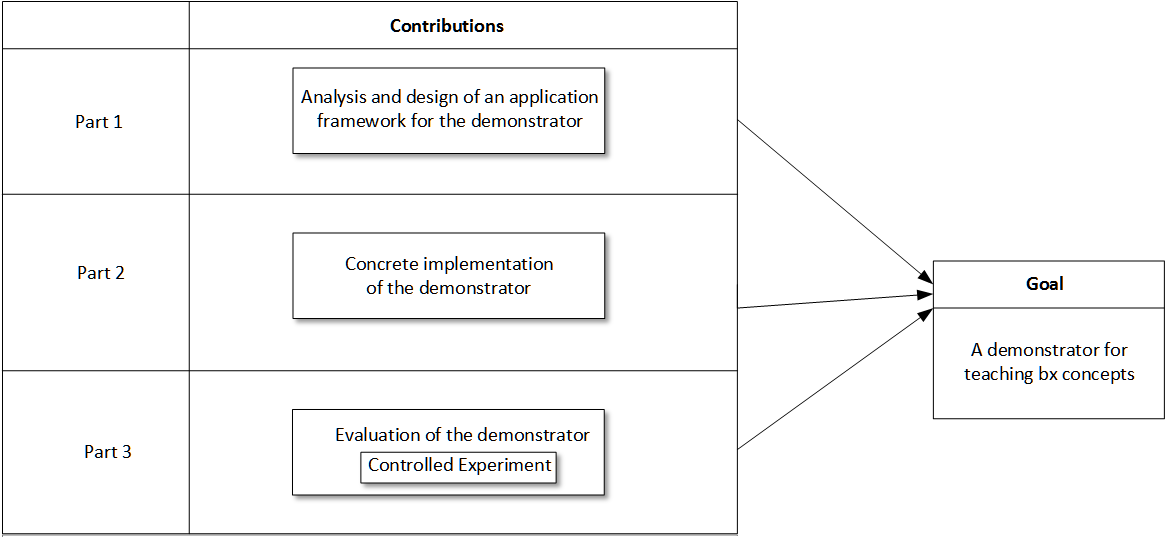
\includegraphics[width=1\textwidth]{figures/Contribution}
	\caption{Contributions}
	\label{fig:Contribution}
\end{figure}

Besides giving an overview of previous work and comparing their advantages and disadvantages with my demonstrator, Figure~\ref{fig:Contribution} shows my contributions towards providing a solution to the problems described in Section \ref{subsec:probstmt}. It can be categorized into three parts: 

\begin{enumerate} 
	\item {Analysis and design of an application framework for the demonstrator} 
	\item {Concrete implementation of the demonstrator}
	\item {Evaluation of the demonstrator}
\end{enumerate}

After analyzing the existing work on bx and their related problems (detail explanation described in Section \ref{sec:relatedwork}), to solve the problems in hand, designing an application framework for the implementation of an interactive demonstrator was needed. Hence, I have designed a working, fully functional application framework based on MVC pattern for implementing a bx tool demonstrator along with an interactive user interface for the accomplishment of point (1). This framework can be used to implement a demonstrator encapsulating bx tools with concrete examples.

Along with this achievement, a concrete implementation of a demonstrator to check the feasibility and validity of the application framework was needed. Hence, I have implemented a fully functional online demonstrator (\textit{\ac{Demon-BX}}) based on the application framework designed earlier for the accomplishment of point (2). This demonstrator is based on a bx tool i.e., eMoflon and a concrete example leveraging the functionalities of the bx tool and explaining some basic bx concepts. 

After the implementation, evaluation of the demonstrator to check the effectiveness and its impact on the mass audience was needed. Hence, I have evaluated the demonstrator based on the research method called controlled experiments \cite{semethods} for the accomplishment of point (3). This experiment was based on three hypotheses, which helped in deciding which variables i.e., dependent, independent, and controlled to include and how to measure them. A well-designed experiment was performed with two different groups of participants and collected data were analyzed to measure the outcome.

All of my contributions help to achieve the goal of this thesis i.e., a demonstrator for teaching bx concepts.

\subsection{Structure of Thesis}\label{subsec:structure}

Chapter 1 (Introduction) contains the introduction and motivation about the thesis with a solution strategy. Chapter 2 discusses the related terminologies with respect to bidirectional transformation. Chapter 3 describes the requirements for implementing a successful bx demonstrator. Chapter 4 explains the related work that has been done on bx in the last few years and their related problems. Chapter 5 describes all the high-level design and implementation details for the demonstrator along with UML diagrams. Chapter 6 contains the evaluation methodology and evaluation results. The last chapter summarizes all the work which was done as part of this thesis and draws conclusions followed by future work.

\clearpage
\section{Foundation}\label{sec:foundation}
This chapter provides an overview of my running example in Section \ref{subsec:runningexample} followed by definitions of some commonly used terminologies with respect to bx in Section \ref{subsec:definitions}. This chapter will lay the foundation for understanding the basics for the reader and will help him/her in apprehending the concepts explained in further chapters.

In this thesis, bidirectional transformation will be discussed by referring to a \textit{Kitchen Model} and a \textit{Grid Model} of a software system. Both models describe the structure and behavior of the real system "kitchen" but from different perspectives.

\subsection{Running Example}\label{subsec:runningexample}
This example is a simplified kitchen planner. Figure~\ref{fig:Running_Example_GUI} describes the relation between the \textit{Kitchen Model} denoted by \textit{Kitchen} (right-hand side canvas) and the \textit{Grid Model} denoted by \textit{Layout} (left-hand side canvas). 

\begin{figure}[h]
	\centering
	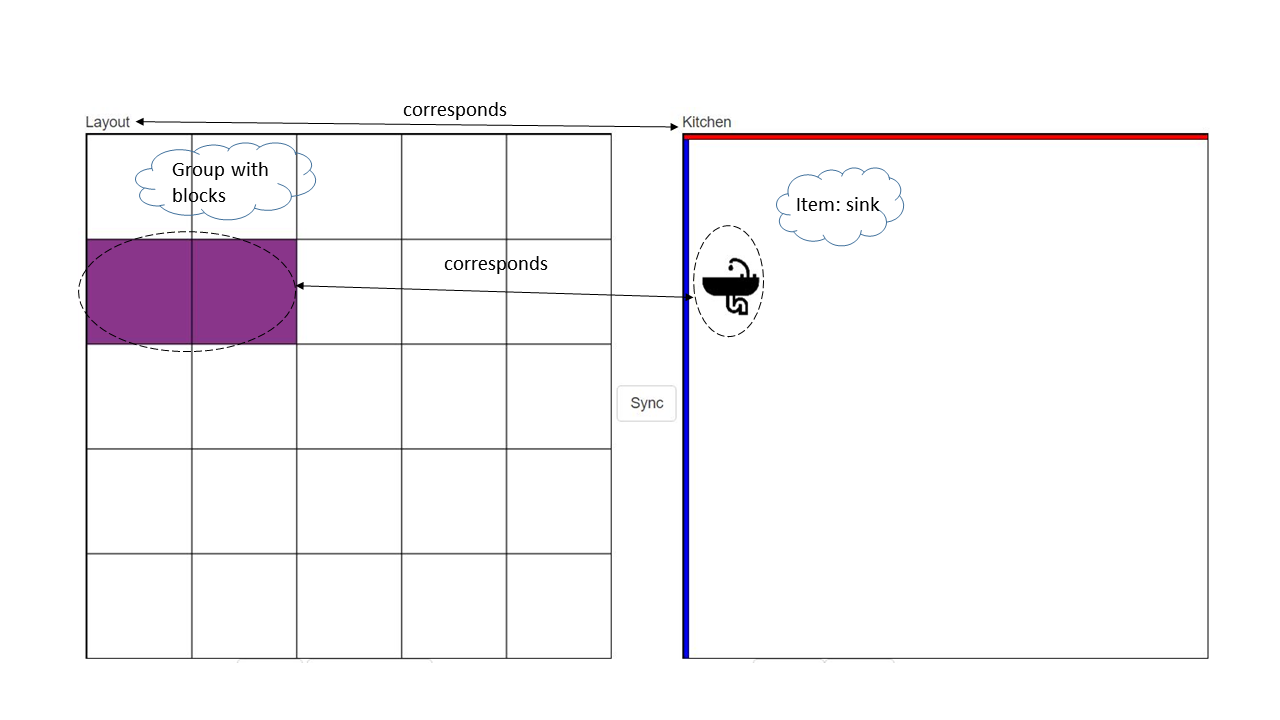
\includegraphics[width=1\textwidth]{figures/KitchenToGrid}
	\caption{Running Example: Layout and Kitchen}
	\label{fig:Running_Example_GUI}
\end{figure} 

\begin{figure}[h]
	\centering
	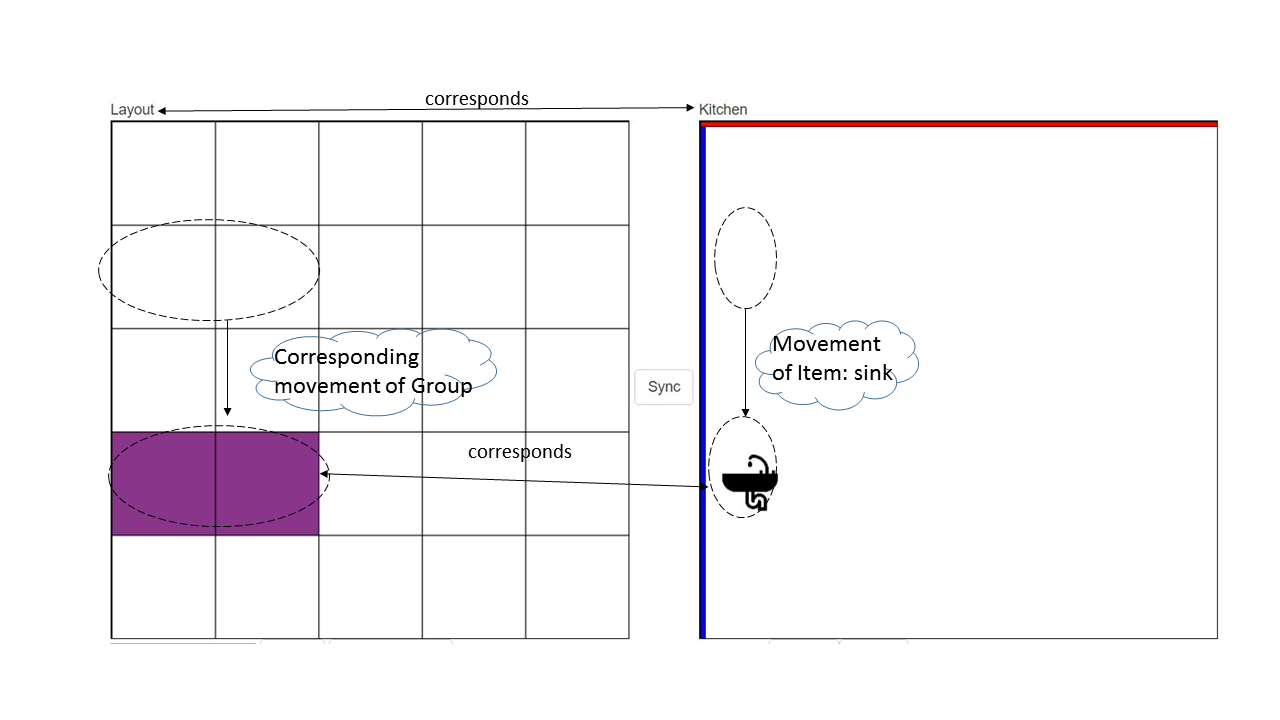
\includegraphics[width=1\textwidth]{figures/KitchenToGrid_consistency}
	\caption{Running Example: Consistency Preservation}
	\label{fig:Running_Example_GUI_consistency}
\end{figure}

\textit{Kitchen} contains items e.g., sink, fridge, table etc. You can create, delete or move these items in the kitchen, and press "Sync" to propagate your changes to the layout. The \textit{Layout} consists of groups of a certain number of blocks. This shows how much space the objects occupy as colored groups of blocks organized in a grid. Here, the \textit{Kitchen} corresponds to the \textit{Layout} and a single \textit{Item} corresponds to a \textit{Group}. This is described in Figure~\ref{fig:Running_Example_GUI} where an item e.g., \textit{sink} created in the \textit{Kitchen} corresponds to a group in the \textit{Layout}.

Both artifacts are created and evolve together during the lifecycle of the application representing a kitchen workspace. Thus, changes in one domain should be propagated to the other domain in order to ensure consistency between these related artifacts. This is shown in Figure~\ref{fig:Running_Example_GUI_consistency}.

Model transformation and synchronization is discussed with this scenario throughout this thesis. 

\subsection{BX Basics}\label{subsec:definitions}

\begin{defn}\label{defModel} (Model and Meta-Model)\\
A model depicts the structure and/or behavior of a real system under discussion from a certain point of view and at a certain level of abstraction which helps in managing and understanding the complexities of a system \cite{uml} \cite{mdsd}. Model creation helps in keeping a clear focus on selected concepts and rules relevant for a particular concern and omitting irrelevant details.

A metamodel describes a set of models, i.e., defines a modeling language. 
\end{defn} 

\begin{table}
	\centering	
	\begin{tabular}{|p{3cm}|p{3cm}|p{8cm}|}
		\hline
		\rowcolor[gray]{.8}	
		\textbf{Reality} & \textbf{Model} & \textbf{Aspects Covered} \\
		\hline
		Kitchen & Kitchen Model & 
		\begin{itemize}
			\item Area of a kitchen as a white space
			\item 4 walls of a kitchen
			\item Contains the objects of a kitchen
			\item Creation, movement, deletion of kitchen objects
		\end{itemize}\\
		\hline
		Kitchen & Grid Model & 
		\begin{itemize}
			\item Area of a kitchen as a block structure
			\item 4 walls of a kitchen
			\item Contains the objects of a kitchen
			\item Creation, deletion of kitchen objects
		\end{itemize}\\
		\hline					
		
	\end{tabular}
	\caption{Model and Reality}
	\label{tab:Model_Reality}
\end{table}

\textit{Example:} In my demonstrator, the example that I have two meta-models i.e., \textit{Kitchen} and \textit{Grid}. Both the models represent the reality "Kitchen". A relation between reality and models is shown in Table~\ref{tab:Model_Reality}. 

Figure~\ref{fig:Grid_MetaModel} and Figure~\ref{fig:Kitchen_MetaModel} depict the \textit{Grid} and \textit{Kitchen} meta-model respectively as a class diagram from an object oriented point of view showing the related classes and the relationship between them.

\begin{figure}[h]
	\centering
	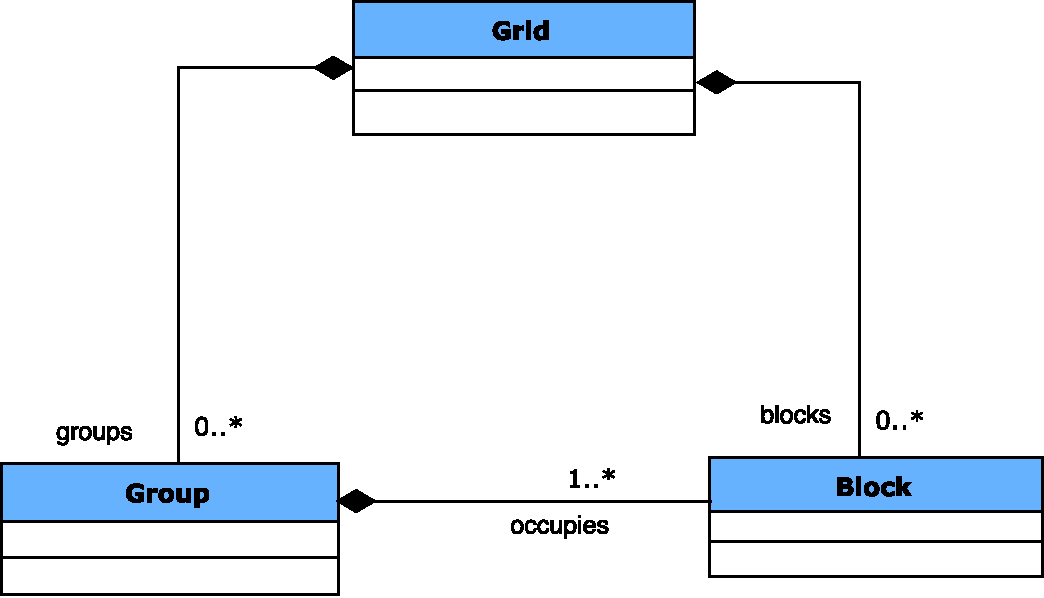
\includegraphics[width=0.7\textwidth]{figures/Grid_MetaModel}
	\caption{Grid MetaModel}
	\label{fig:Grid_MetaModel}
\end{figure}

\begin{figure}
	\centering
	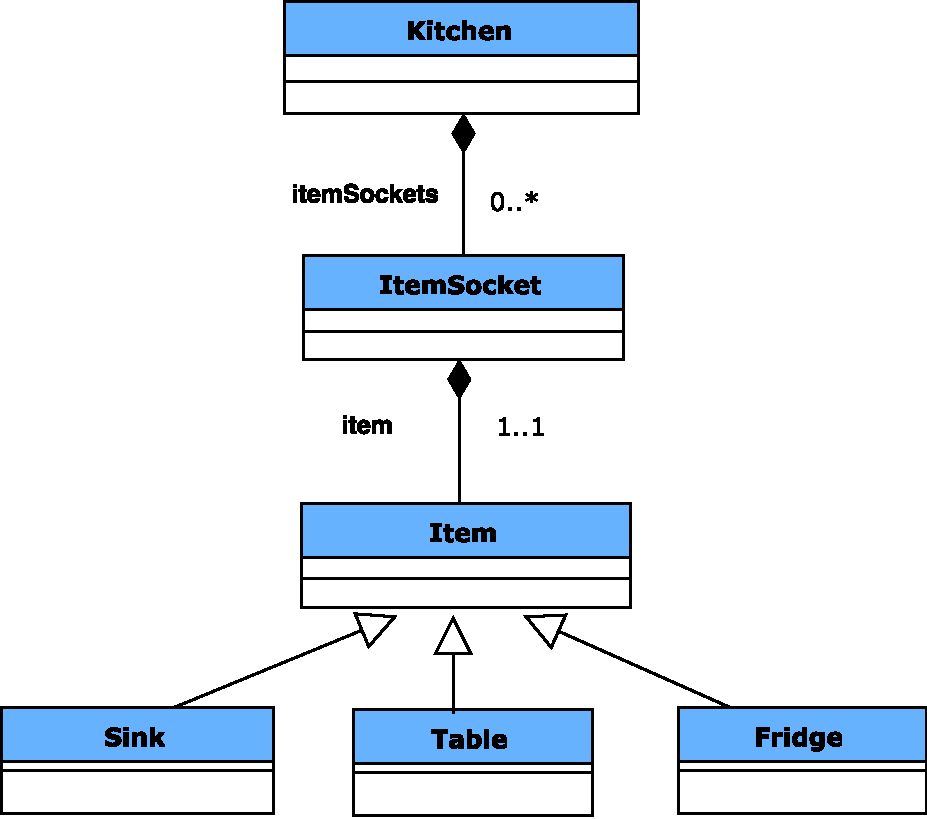
\includegraphics[width=0.7\textwidth]{figures/Kitchen_MetaModel}
	\caption{Kitchen Meta-Model}
	\label{fig:Kitchen_MetaModel}
\end{figure}

Figure~\ref{fig:Kitchen_AbstractConcrete} illustrates an abstract and concrete view of the \textit{Kitchen} model. The left-side figure shows an abstract syntax i.e., an instance of the kitchen. Whereas, right-side figure describes a concrete syntax of the kitchen as visualized in the user interface.\\

\begin{figure}
	\centering
	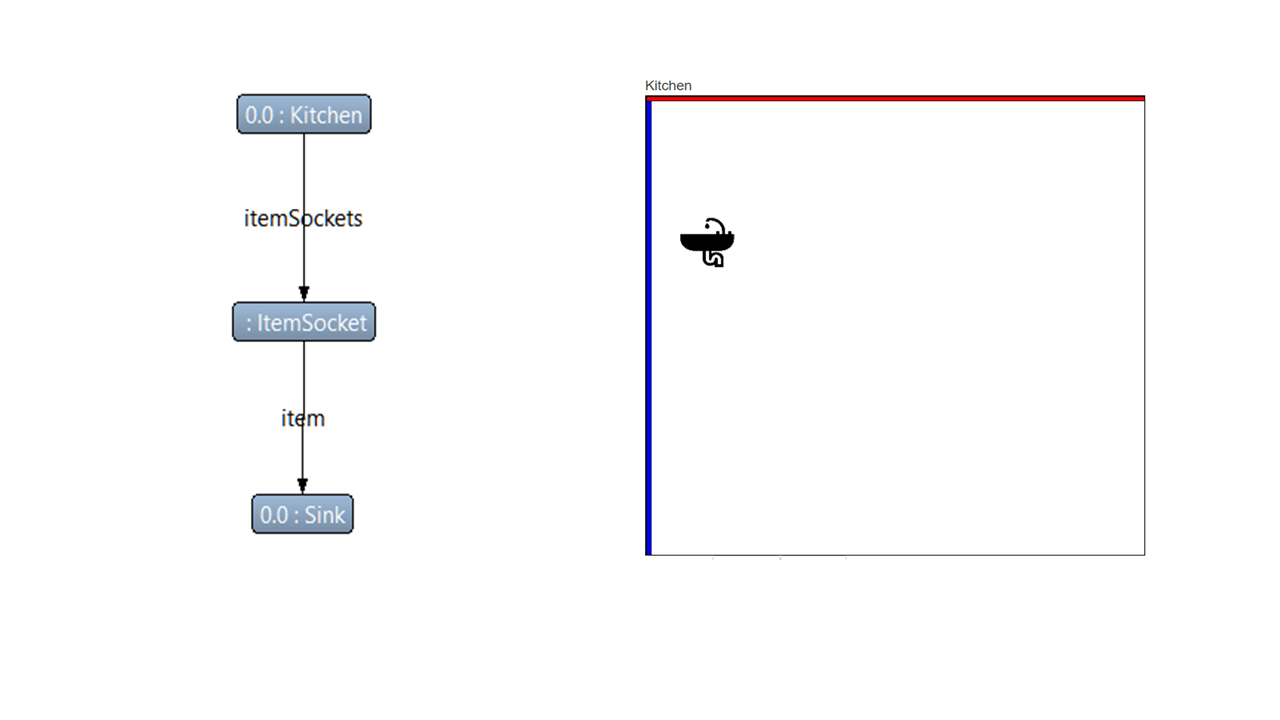
\includegraphics[width=1\textwidth]{figures/Kitchen_AbstractConcrete}
	\caption{Kitchen Model (Abstract \& Concrete)}
	\label{fig:Kitchen_AbstractConcrete}
\end{figure}

\begin{defn}\label{defDelta} (Delta)\\
A delta is a change applied to one or more properties of an artefact. It denotes the relationships between models from the same model space \cite{benchmarx-reload}. It is denoted $\delta$: M $\longrightarrow$ M' where M' is an updated version of M.
\end{defn}

\textit{Example:} In my demonstrator example, deltas related to the "Kitchen Model" are described in Table~\ref{tab:Examples_of_Delta}. Whereas, Figure~\ref{fig:Delta_Propagation} shows a concrete example of delta propagation, where the creation of a new item e.g., sink causes the change from Kitchen to Kitchen'.\\

\begin{table}
	\centering	
	\begin{tabular}{|p{4cm}|p{8cm}|}
		\hline
		\rowcolor[gray]{.8}	
		\textbf{Model} & \textbf{Delta ($\delta$)} \\
		\hline
		Kitchen Model & 
		\begin{itemize}
			\item Creating a new item
			\item Deleting an existing item
			\item Moving an item
		\end{itemize}\\
		\hline				
		
	\end{tabular}
	\caption{Examples of Delta in Kitchen Model}
	\label{tab:Examples_of_Delta}
\end{table}

\begin{figure}
	\centering
	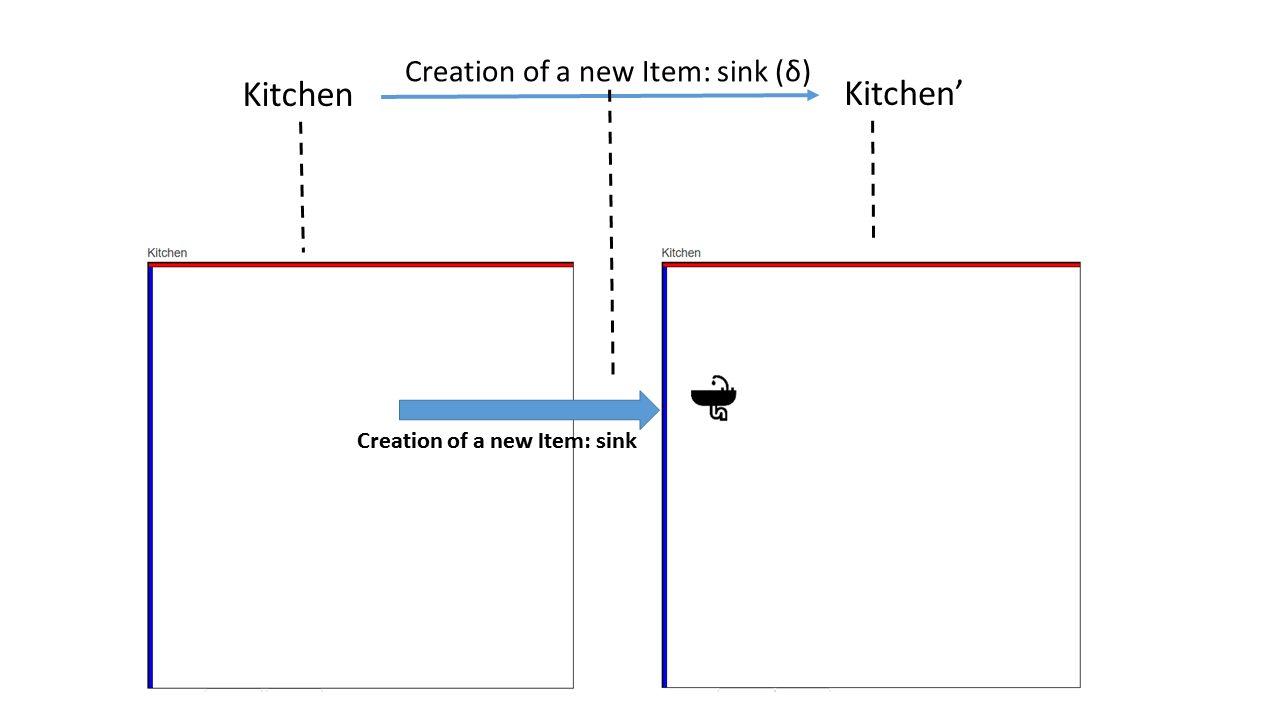
\includegraphics[width=1\textwidth]{figures/Delta_Propagation}
	\caption{Delta Propagation}
	\label{fig:Delta_Propagation}
\end{figure}

\begin{defn}\label{defModelSpace } (Model Space)\\
A Model Space describes all the states of an artefact (models of the same type) and all the deltas which lead from one model to another.
\end{defn}

\textit{Example:} In my demonstrator example, a concrete example of a subset of a model space is shown in Figure~\ref{fig:Model_Space}. GS contains the states i.e., Grid1, Grid2, Grid3 along with deltas i.e., $\delta$1, $\delta$2 of the \textit{Grid} Model. Whereas, KS contains the states i.e., Kitchen1, Kitchen2, Kitchen3 along with deltas i.e., $\delta$3, $\delta$4 of the \textit{Kitchen} Model.

\begin{defn}\label{defCorrespondenceLinks } (Correspondence Links)\\
Relationships between models from different model spaces are called correspondence links, or just corrs \cite{benchmarx-reload}. Corrs are used to relate two model spaces. A corr is a set of links c(a; b) between models (a in A, b in B), where  a, b are models in model spaces A and B respectively.
\end{defn}

\textit{Example:} In my demonstrator example, an example of a corr c(Grid2; Kitchen2) is shown in Figure~\ref{fig:Model_Space}. A concrete example of the corr is given in  Figure~\ref{fig:Correspondence_Links}.

\begin{figure}
	\centering
	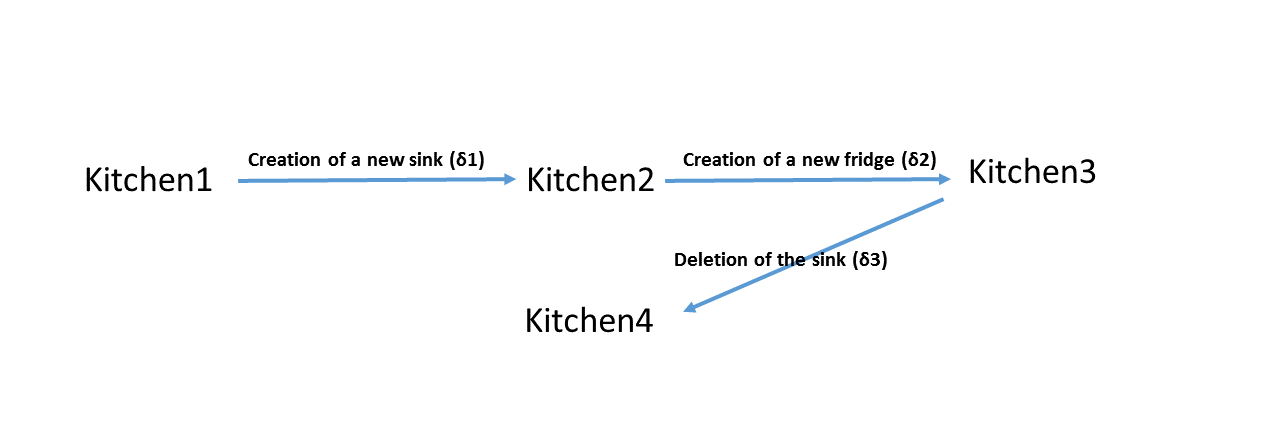
\includegraphics[width=1\textwidth]{figures/Model_Space}
	\caption{Model Space}
	\label{fig:Model_Space}
\end{figure}

\begin{figure}
	\centering
	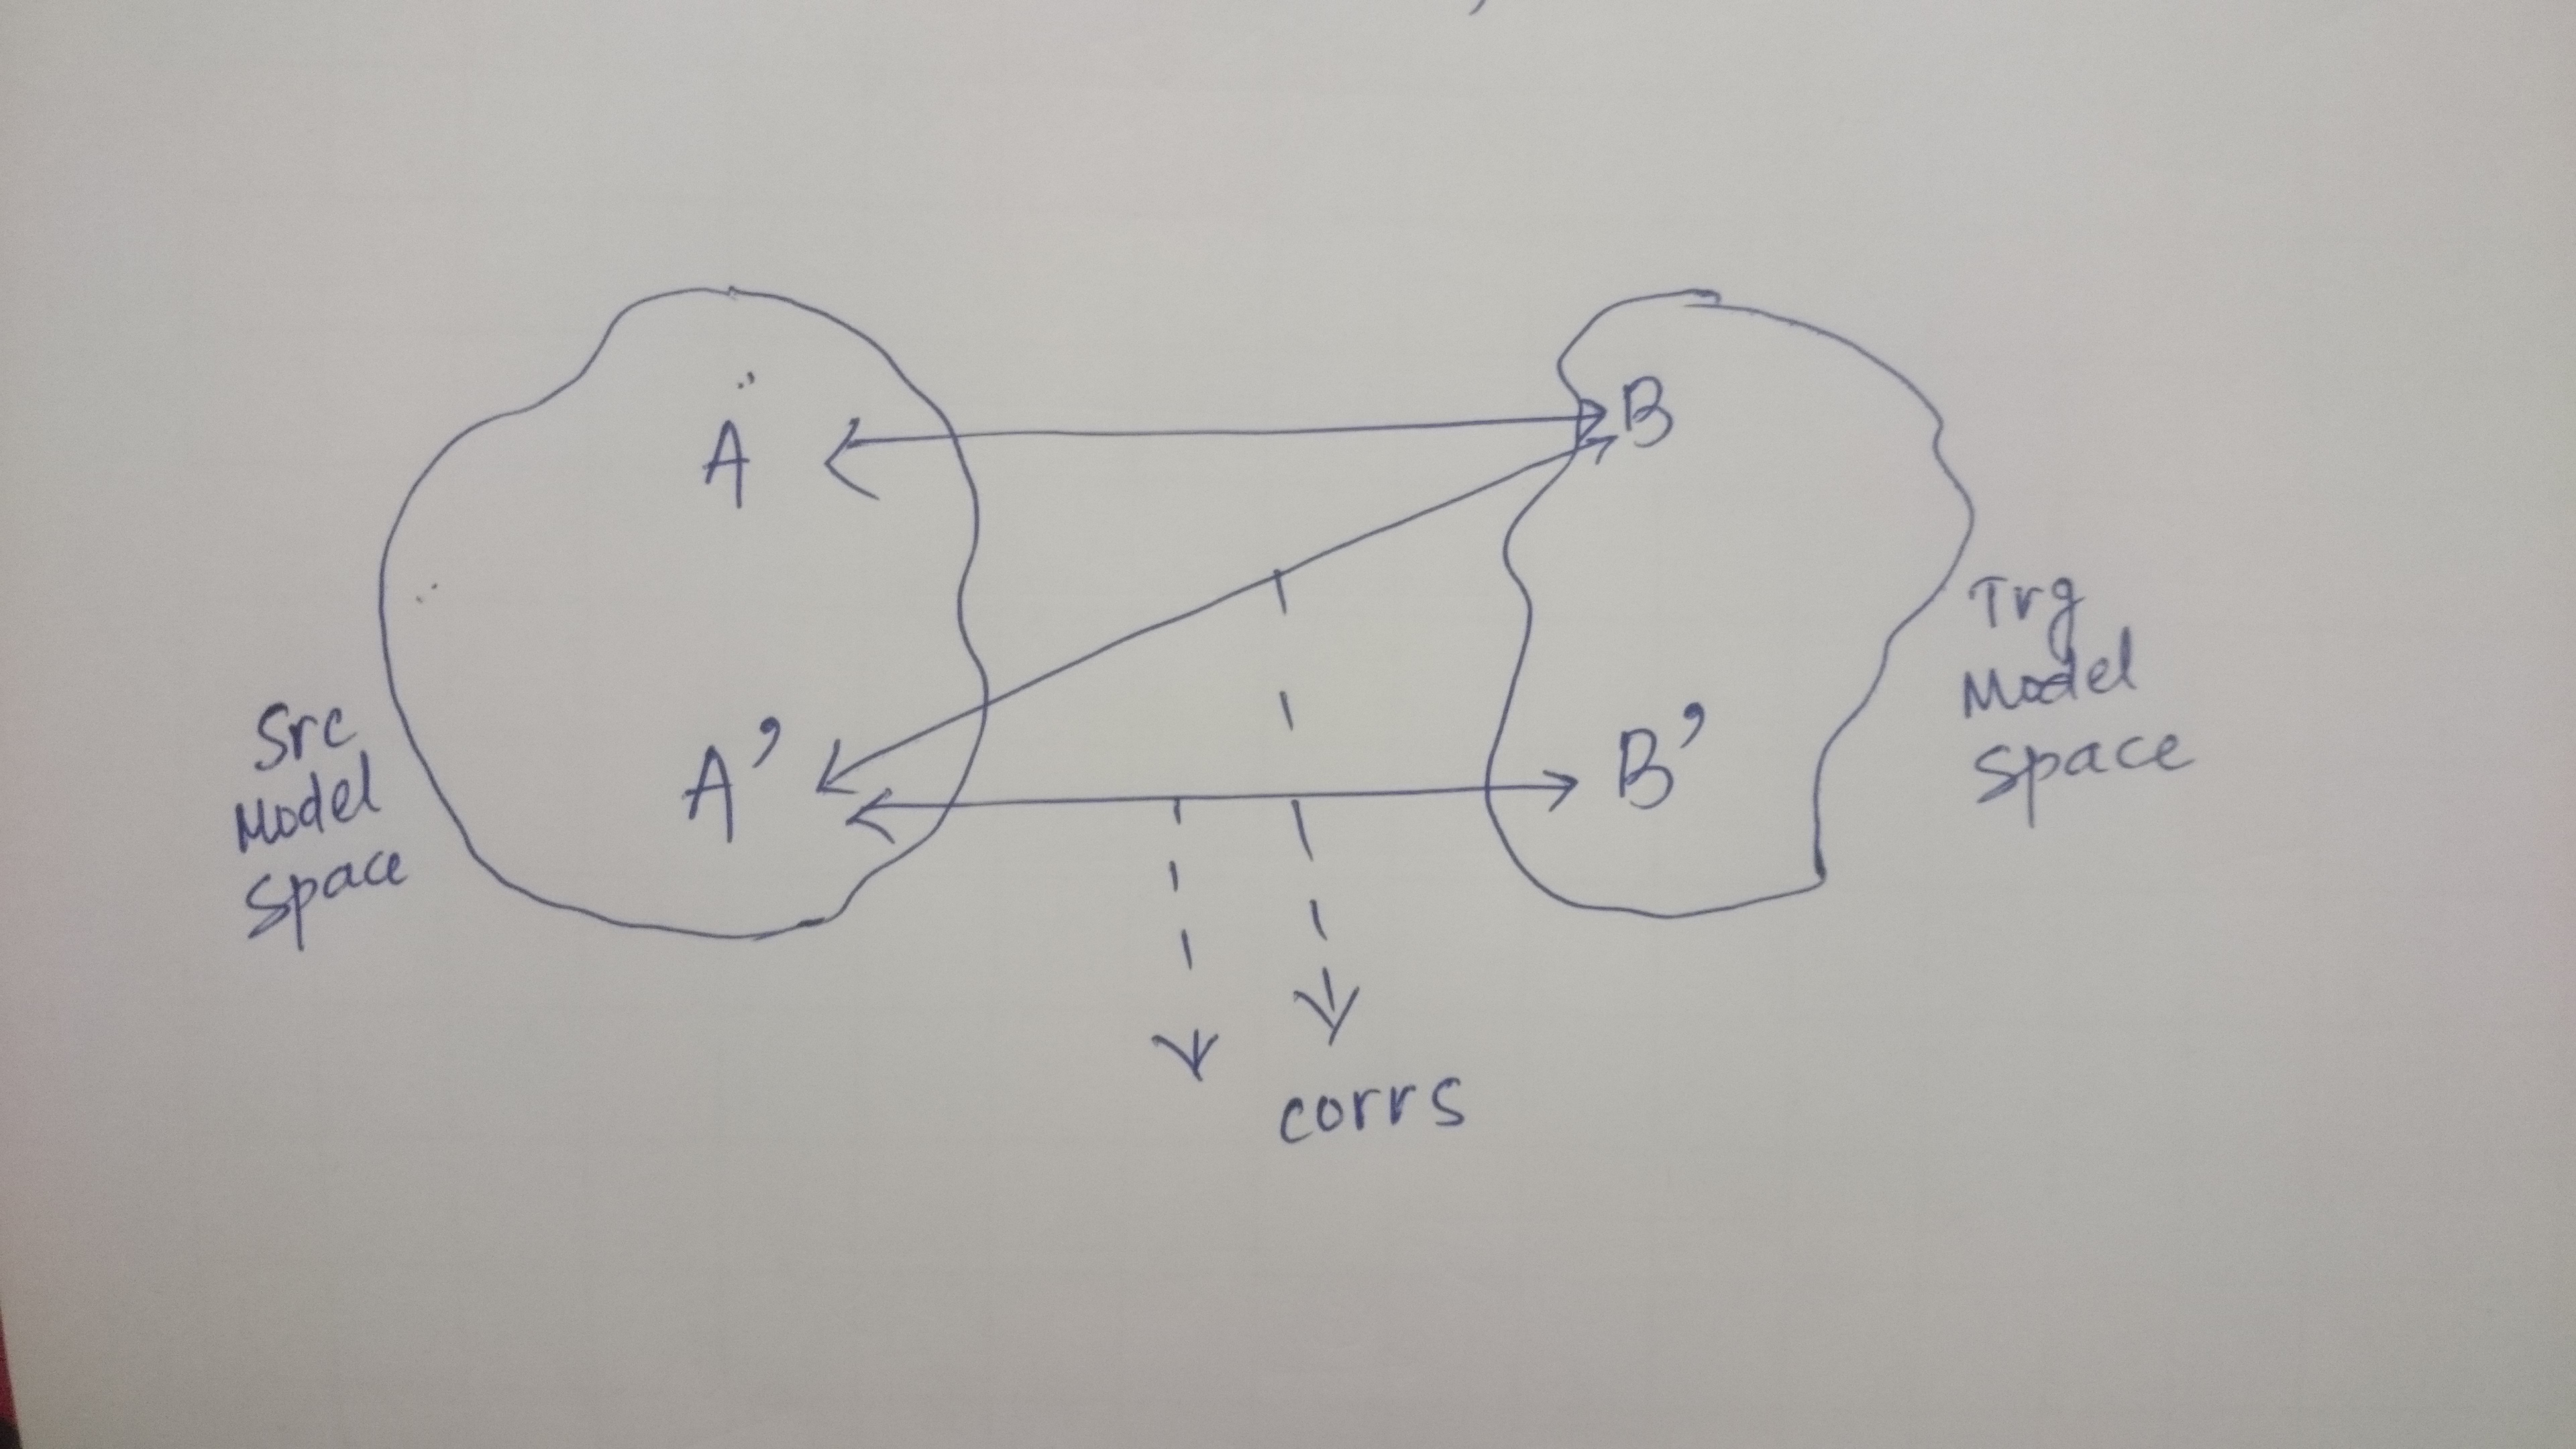
\includegraphics[width=1\textwidth]{figures/Corr}
	\caption{Correspondence Links}
	\label{fig:Correspondence_Links}
\end{figure}

\begin{defn}\label{defConsistency } (Consistency)\\
Changes in one model may or may not cause any change in another correspondence model (model from different model space) but their states must not contain any contradiction. Consistency in model transformation is measured on the correctness and completeness of the operations performed \cite{modelsynchro-tgg}. For example, consistency between two models is ensured when a change in one model causes correct  restoration of all the association/corrs between the models (correctness) and all valid inputs are propagated (completeness).
\end{defn} 

\textit{Example:} In my demonstrator example, a \textit{Kitchen} model is consistent with a \textit{Grid} model when a mapping between \textit{itemSocket} and \textit{group} can be established such that itemSocket containing an item is paired with a group containing block(s). 
Figure~\ref{fig:Running_Example_GUI} and Figure~\ref{fig:Running_Example_GUI_consistency} describe a concrete example of consistency preservation where changes in \textit{Kitchen} (Kitchen model) i.e., movement of the sink should ensure the movement of the corresponding group with two horizontal blocks in \textit{Layout} (Grid model) in order to ensure consistency.

\begin{defn}\label{deffwdbkdtrans} (Forward and Backward Transformation)\\
Model transformation is defined as a process for propagating the changes (deltas) from one model of one domain to a corresponding model in another domain using forward and/or backward transformation operations. After a transformation operation, consistency of source and target model is always ensured as model transformation ensures that for each consistent source model there exist a consistent target model~\cite{modelsynchro-tgg}.

In forward transformation, only the changes that occur in the source model is propagated to the target model ensuring the consistency between source and target model.

In backward transformation, only the changes that occur in the target model is propagated to the source model ensuring the consistency between source and target model.

Given two models, the bidirectional transformation is a pair of transformation which takes place in both forward and backward direction maintaining the consistency relation between them~\cite{understanding-bx}.
\end{defn}

\textit{Example:} In my demonstrator example, "Grid" is the \textit{Source} model and "Kitchen" is the \textit{Target} model. Forward transformation will cause "Grid Model" to transform into "Kitchen Model" and Backward transformation will cause "Kitchen Model" to transform into "Grid Model".

\begin{figure}
	\centering
	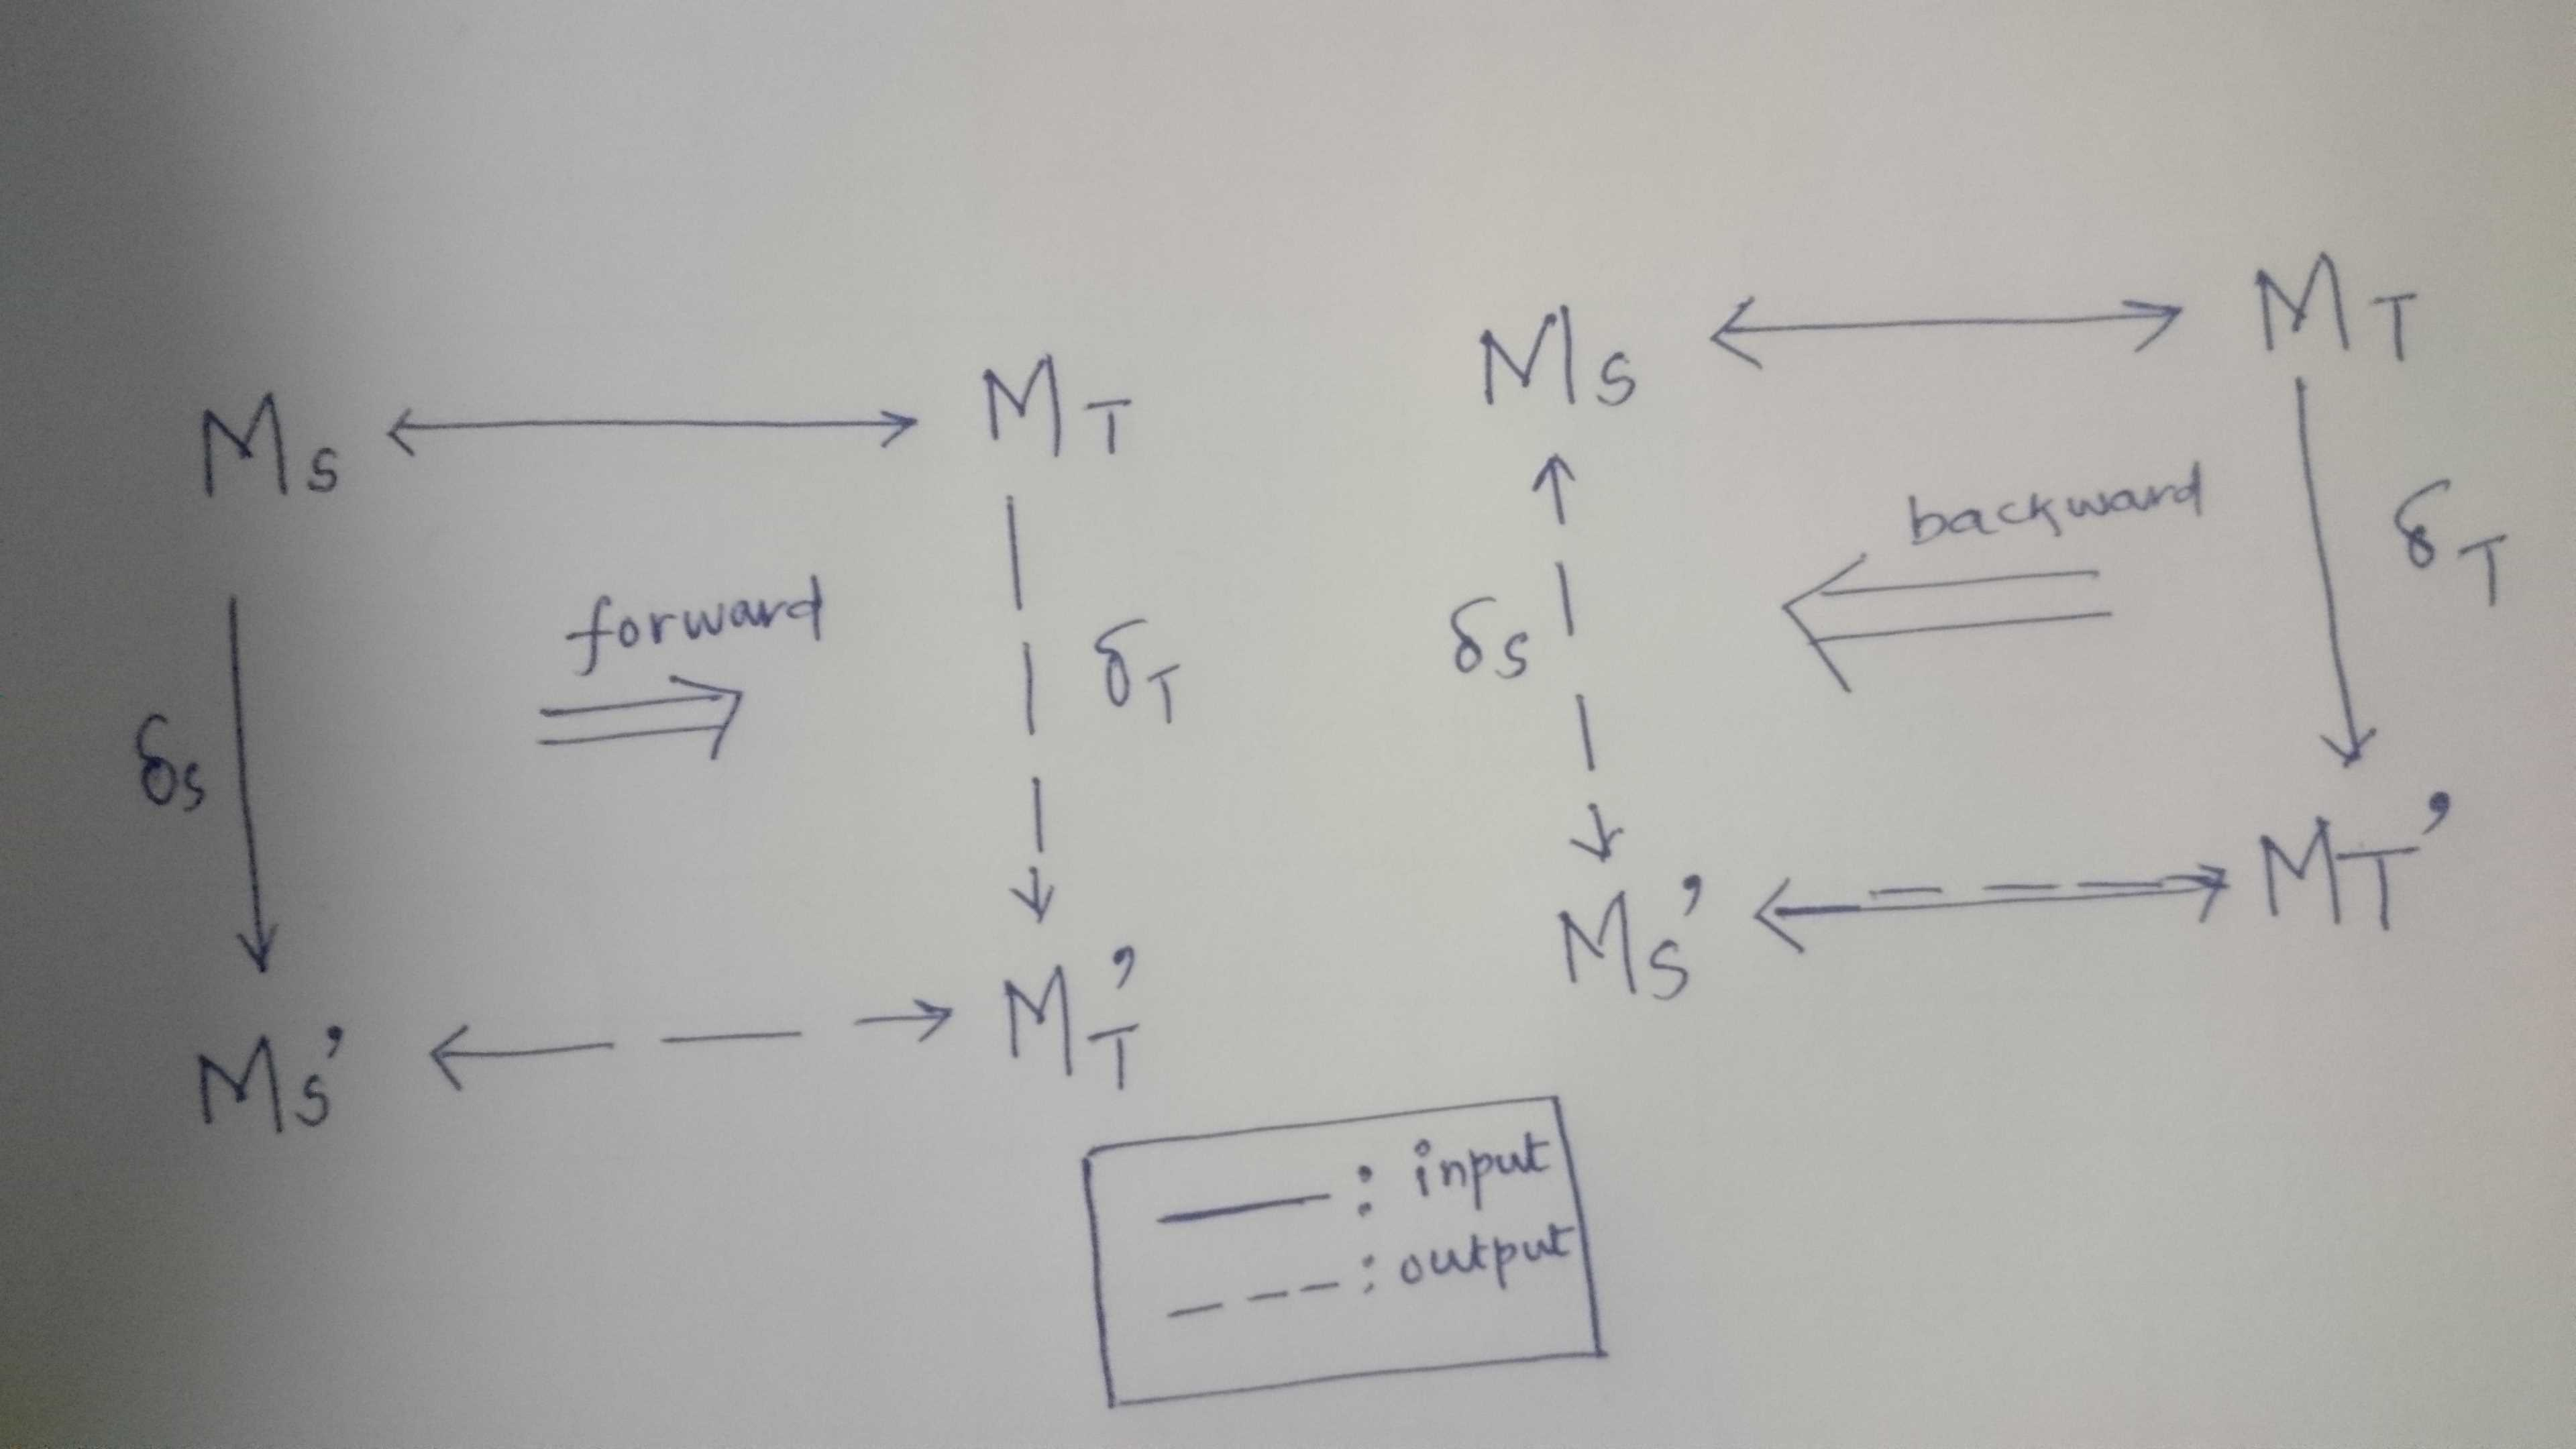
\includegraphics[width=1\textwidth]{figures/BX}
	\caption{Bidirectional Transformation}
	\label{fig:BX_Diagram}
\end{figure}

\begin{figure}
	\centering
	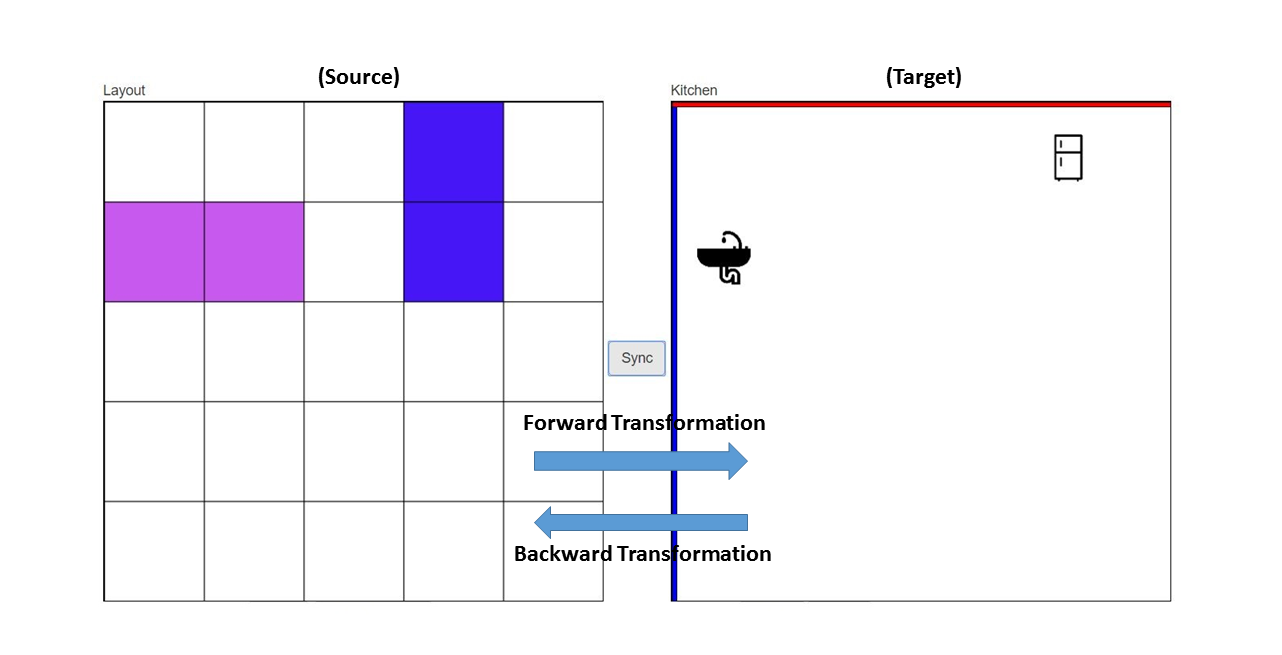
\includegraphics[width=0.8\textwidth]{figures/Transformation_Concrete}
	\caption{Transformation (Concrete Diagram)}
	\label{fig:Transformation_Concrete}
\end{figure}

Figure~\ref{fig:BX_Diagram} shows an abstract example of the "BX" describing both forward and backward transformation. Whereas, Figure~\ref{fig:Transformation_Concrete} depicts a concrete example of the "BX" process where \textit{Layout} and \textit{Kitchen} are described as source and target respectively in the process of forward and backward transformation.
  	\newpage
  	\section{Related Work}\label{sec:relatedwork}
This chapter sums up all the related work that has been done on bx. Section \ref{subsec:handbook}, \ref{subsec:examplerep}, \ref{subsec:existingdemo} and \ref{subsec:virtualmachines} describe the various ways that bx community and developer's group have tried to make the work done on bx visible to the world. Then, Section \ref{subsec:problem} explains the related problems. 
\newline\newline Model transformation is a central part of Model-Driven Software Development \cite{bx-grace} \cite{bx-dagstuhl}. Bx community has been constantly doing research and development work in many fields to help people understand and increase awareness about bx. Nowadays, researchers from different areas are actively investigating the use of bx to solve a variety of problems. A lot of work has been done in terms of building usable tools and languages for bx. These tools can be used in various fields, for achieving \textit{bidirectional transformation}. To understand these tools, several handbooks, tutorials and examples have been created so that users and developers can understand the core concepts. 
\subsection{Handbooks \& Tutorials}\label{subsec:handbook}
As a part of our research, I have analyzed some tutorials and tools and below are my findings.
\newline\newline Anjorin et al.\cite{emoflon-part4} present the concept for \textit{bidirectional transformation} using Triple Graph Grammars (denoted by "TGG") \cite{tgg}. To demonstrate their core idea and the usage of the tool, they have described an example by transforming one model (source) into another (target) through TGG transformations \cite{tgg}\cite{bx-tgg}. The whole tutorial is about 42 pages long which guides the user to get the example running through a series of steps. These steps include installing \ac{Eclipse}, getting their tool as an Eclipse plugin, setting up the workspace, creating TGG schema and specifying its rule and much more. If the user is able to execute each step correctly, then finally he/she can view the final output. It took me 4 days to get the tool up and running.
\newline\newline We have analyzed a tutorial\cite{bigul-tutorial} on a bidirectional programming language BiGUL\cite{bigul}. The core idea with BiGUL is to write only one putback transformation, from which the unique corresponding forward transformation is derived for free. The whole tutorial is about 45 pages long which includes a lot of complex formulas, algorithms and guides the user to get the example running through a series of steps. These steps include installing BiGUL, setting up the environment, achieving bx through BiGUL's bidirectional programming and much more. If the user is able to execute each step correctly, then finally he/she can view the final output. 

\subsection{Example Repositories}\label{subsec:examplerep}
A rich set of bx examples repository \cite{bx-examples} has been created based on many research papers. These examples cover a diverse set of areas such as business process management, software modelling, data structures, database, mathematics and much more.
\newline\newline User can find relevant information about the examples on the respective web pages. Some of the examples are very well documented along with class diagrams, activity diagrams, object diagrams etc. and source code of a few examples are available as well.

\subsection{Existing Demonstrators}\label{subsec:existingdemo}
Also, we have analyzed an existing demonstrator available along with the test cases of a domain-specific language, BiYacc \cite{biyacc} which is based on BiGUL \cite{bigul}. 
\newline\newline Being an online demonstrator, a user can try it out instantly and check how it works. It doesn't require any installation or technical expertise to get the example running and also, it makes the features of bx noticeable.
 
\subsection{Virtual Machines}\label{subsec:virtualmachines}
Also, we have analyzed a web-based virtual machine, e.g., SHARE \cite{share}. Basically, this is a web portal used for creating and sharing executable research papers and acts as a demonstrator to provide access to tools, softwares, operating systems, etc., which are otherwise a headache to install \cite{share}. 
\newline\newline This provides the environment that the user requires to execute his/her tool or program. Hence, it reduces the overhead of a user for maintaining and organizing all software framework related stuff and simplify access for end-users.
	
\subsection{Related Problems}\label{subsec:problem}
Some associated problems that I found with the above paragraphs are as follows: 

\begin{itemize}
    \item {Installation requires technical expertise and time consuming as the user typically has to setup and install the tool.}

	\item {Steps to get the example running needed technical expertise, e.g., In some cases domain specific knowledge includes mathematics and specific coding language. What is showcased and discussed is tied to a specific technological space and might not be easily transferable to other bx approaches.}
	
	\item {Not very helpful to understand what bx is before deciding which bx tool (and corresponding technological space) to use.}
	
	\item {The existing demonstrator's visual representation doesn't create interest in the target audience as it does not exploit the potential of using an interactive GUI and colors, etc. It just makes use of two text fields and is comparable to a console-based interface that is accessible online.}
	
	\item {The existing demonstrator is based on a rather technical example that might not be relevant, interesting, or convincing for a large group of potential bx users.}	
	
	\item {For security reasons, virtual machines are not like other web portals where a user need to simply sign-up and can host/create/access data, rather it includes a series of request-grant cycle for getting access to an environment and hosting/managing data. Also, some actions require special authorization and take time to complete the whole process.}

\end{itemize}

  	\newpage
  	\section{Requirements}\label{sec:requirements}
This chapter explains all the research work that I have done before or during the actual implementation. Section \ref{subsec:implementationphases} describes the phases I went through during my thesis work and the research involved. Afterwards, Section \ref{subsec:objectives} deals with the actual research questions I am going to explore during my thesis. Then, Section \ref{subsec:learninggoals} and \ref{subsec:endresult} describes the learning goals for the user and what to expect from the thesis at the end respectively. 

\subsection{Implementation Phases}\label{subsec:implementationphases}
My work is based on an \ac{evolutionary case study} which focuses on designing and implementing a successful bx tool demonstrator. My entire work cycle is described in the following paragraphs.
\paragraph{Case Study}
Initially, the case study was based on the existing work/research done on bx, existing tools available in the market, flexibility in usage, time and technical expertise required to use these bx tools, and the implementation of these tools in different areas. With the initial study and knowledge gathered, I have formulated a few research questions as described in Section \ref{subsec:objectives} in order to evaluate them in my thesis and improve the existing situation and the usefulness of a bx-tool based demonstrator. 
\newline\newline Next step was to choose a bx-tool for my demonstrator. Based on the gathered information and taking account implementation related issues, I have finally chosen a bx-tool to be used as a part of the demonstrator to realize bx. Kindly refer Section \ref{subsec:bxtoolselection} for detailed explanation on bx-tool selection.
\newline\newline Along with the research questions, I have also prepared some learning goals as described in Section \ref{subsec:learninggoals} which the user needs to learn/understand about bx and the bx-tool while playing with the demonstrator.
\paragraph{Examples and Implementation}
Initially, I have constructed a few examples which can be implemented covering the requirements and showing the usability of bx tools through demonstrator and finally chose the best suitable example to implement and build the final prototype. Section \ref{subsec:examples} describes list of all the examples.
\newline\newline Next step was to set up the entire application framework for implementing the demonstrator. First, I did some research by going through materials on software design patterns and web application architecture. Then, I prepared a few proof of concepts(POC) for checking the feasibilty of the architecture designs before finalising my application framework. Kindly refer Section \ref{subsec:concretedesign} for detailed explanation on finalizing the architecture design.
\paragraph{Evaluation} To evaluate the demonstrator, I have conducted a few feedback sessions ....
\newline\newline Based on the feedbacks from the users, .... Kindly refer Section \ref{sec:evaluation} for detailed explanation on evaluation and feedback.
\paragraph{Choices and Threats} 
The implementation process and the final prototype was driven by many choices and threats. For example, 
\begin{itemize} 
	\item {selection of the bx tool and the most suitable example to implement has impact on deciding the usefullness of the demonstrator.}
	\item {seletion of the bx tool and the example to implement is more or less influenced by the ideas given by my supervisor.} 
	\item {my decisions on designing the application's framework for implementation are impacted by the existing availability and usability issues of the finalized bx-tool.}
	\item {During evaluation, I might not have got proper feedback from my friends \& colleagues due to my acquaintance and time constraints.}
\end{itemize}

\subsection{Objectives}\label{subsec:objectives}
The goal of this thesis is to explore the fundamental and technical challenges involved in implementing a demonstrator for bx tools.
\newline\newline This thesis aims at answering these main research questions:
\\\textbf{\textit{RQ1}} -- What are the core requirements for implementing a successful bx demonstrator ?\\
\\\textbf{\textit{RQ2}} -- What kind of interactivity and to what extent is it required in the bx demonstrator ?\\
\\\textbf{\textit{RQ3}} -- Which goals can be particularly well addressed in a bx demonstrator and why ?\\
\\\textbf{\textit{RQ4}} -- To what extent is such a bx demonstrator reusable?\\
RQ4 can be split into the following sub-questions:
\\\textbf{\textit{RQ4.1}} -- Is the implementation of the demonstrator bx tool-specific ?\\
\\\textbf{\textit{RQ4.2}} -- Is the implementation of the demonstrator example-specific?\\
\\\textbf{\textit{RQ4.3}} -- What part(s) of the demonstrator can be reused in implementing a different example ?
\newline\newline All of my work is directly or indirectly related to the above research questions.

\subsection{Learning Goals}\label{subsec:learninggoals}
Along with exploring the challenges as described in Section \ref{subsec:objectives}, I am also focussing on teaching some basic concepts to the user about bx in the process of trying/playing with the demonstrator.

What am I trying to teach?
\begin{itemize} 
	\item {Bidirectional is not always bijective.} 
	\item {Not all changes can be propagated. In this case, consistency needs to be preserved.}
	\item {In BX, Challenge is to avoid or minimise information loss.}
	\item {Current limitation - you can only change one side.}
	\item {Synchronisation is interactive (to handle non-determinism).}	
\end{itemize}

\subsection{End Result}\label{subsec:endresult}
As my thesis is more focussed on the implementation of a demonstrator for consistency management based on a bx tool, following are the end results I am trying to achieve:
\begin{itemize} 
	\item {Reduce the installation time of the bx tool by making the demonstrator available online. Hence, the user is just a click away to try the bx tool and needs nothing to install on his/her machine.} 
	\item {Demonstartor should be interactive and fun to play with.}
	\item {User should be able to learn/understand the concepts of bx as described in Section \ref{subsec:learninggoals}.}
\end{itemize}












  	\newpage
  	\section{High-Level Concepts}\label{sec:highlevel}
In this chapter, I am going to describe all high-level technical details realized during the implementation of the demonstrator. Section \ref{subsec:examples} describes all the examples that I have conceptualized before choosing the final one for the implementation. This is then followed by
the description of the steps taken for selecting the bx-tool in Section \ref{subsec:bxtoolselection}. Afterwards, Section \ref{subsec:concretedesign} deals with the decisions taken for finalizing the apllication's architecture design.
\subsection{Choosing an Example}\label{subsec:examples}
Due to the existing pain points with the bx tools, as described in Section \ref{subsec:motivation} and to solve the problems as described in Section \ref{subsec:problem}, the main idea is to design and implement an interactive bx tool demonstrator.
I have constructed a few examples for implementation as follows:
\paragraph{Task Management} This prototype can be used for allocating tasks in a team. It contains two views e.g., supervisor's view and employee's view. A Supervisor can allocate tasks to their subordinates. An employee can view the tasks assigned to him. Then the task will go through a life cycle as the work progresses, i.e., Assigned, In Progress, Testing, Done. Supervisor's view shows aggregate information from multiple projects and multiple employees, but does not contain detailed information, e.g., tasks have fewer states than for assigned employees. Bx rules control how updates are handled and states are reflected in the different views of the project, e.g., the employee's view will be updated for each state change, whereas the supervisor's view is only updated when a task is completed and not for intermediate changes.

\paragraph{Quiz} This prototype can be used for an online quiz game. It contains two views e.g., administrator's view and participant's view.
There will be a large set of questions related to different areas, e.g, history, geography, politics, sports, etc. The administrator can select the areas from which the questions will be shown to the participant and initiate the game. The participant can override the selection of the areas and start the quiz. Randomly questions will be shown to the participant from the selected areas with 4 options. The administrator's view contains less information than the participant's view, e.g., only the result of each question will be shown to the administrator, whereas participant can see questions along with its options. As soon as the participant chooses the answer to any question, bx rules control how updates are handled and states are reflected in the different views of the project.

\paragraph{Playing with Shapes} It contains two views e.g., low-level view (depicts \ac{UI} for low-level language, i.e., UI with less functionality) and high-level view (depicts UI for high-level language, i.e., UI with more functionality). User will draw a geometric shape, i.e., triangle / square / rectangle / circle with some notations similar to the shape on the low-level view and if the notations are correct, the high-level view tries to recognize the shape and draws it with default parameters and vice-versa. Basically the transformation will happen between a low-level language and a high-level language and bx rules control how updates are handled and states are reflected in the different views of the project. In high-level view, more functionalities will be present, i.e., moving one shape from one place to another, creating a clone of an existing shape, etc. which is not possible in low-level view.

\paragraph{Arranging a Kitchen}
It contains two views e.g., low-level view (depicts a grid structure containing blocks) and high-level view (empty space which depicts UI for kitchen). High-level view has more functionalities such as creating/ deleting/ moving an kitchen item, etc. out of which only a few will be available in low-level view. User will create/ delete/ move a kitchen item, i.e., sink / table on the high-level view and if changes done on the high-level view are according to the rules defined in the bx tool then items will be reflected on the low-level view with same colored blocks and vice-versa. Basically the transformation will happen between a low-level language and a high-level language and bx rules control how updates are handled and states are reflected in the different views of the project.

\subsection{BX Tool Selection}\label{subsec:bxtoolselection}

\subsection{Concrete Design Decision and High-Level Architecture Information}\label{subsec:concretedesign}
High-Level Architecture diagram of my prototype is given in Figure~\ref{fig:Architecture_Diagram}.
\begin{figure}
	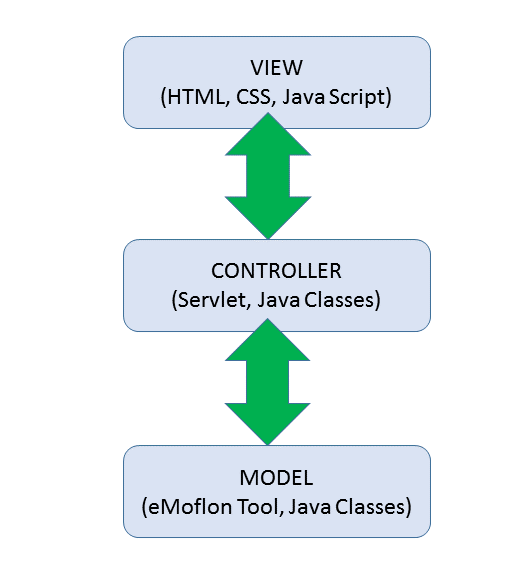
\includegraphics[width=1\textwidth]{figures/Highlevel_Arch}
	\caption{High Level Architecture Diagram}
	\label{fig:Architecture_Diagram}
\end{figure}
\subsubsection{View (GUI)}\label{subsubsec:view}
\subsubsection{Controller}\label{subsubsec:controller}
\subsubsection{Model}\label{subsubsec:model}







  	\newpage
  	\section{Low-Level Concepts}\label{sec:lowlevel}

\subsection{UML Diagrams}\label{subsec:umldiagrams}
\subsubsection{Component Diagram}\label{subsubsec:component}
Component diagram of my prototype is given in Figure~\ref{fig:Component_Diagram}.
\begin{figure}
	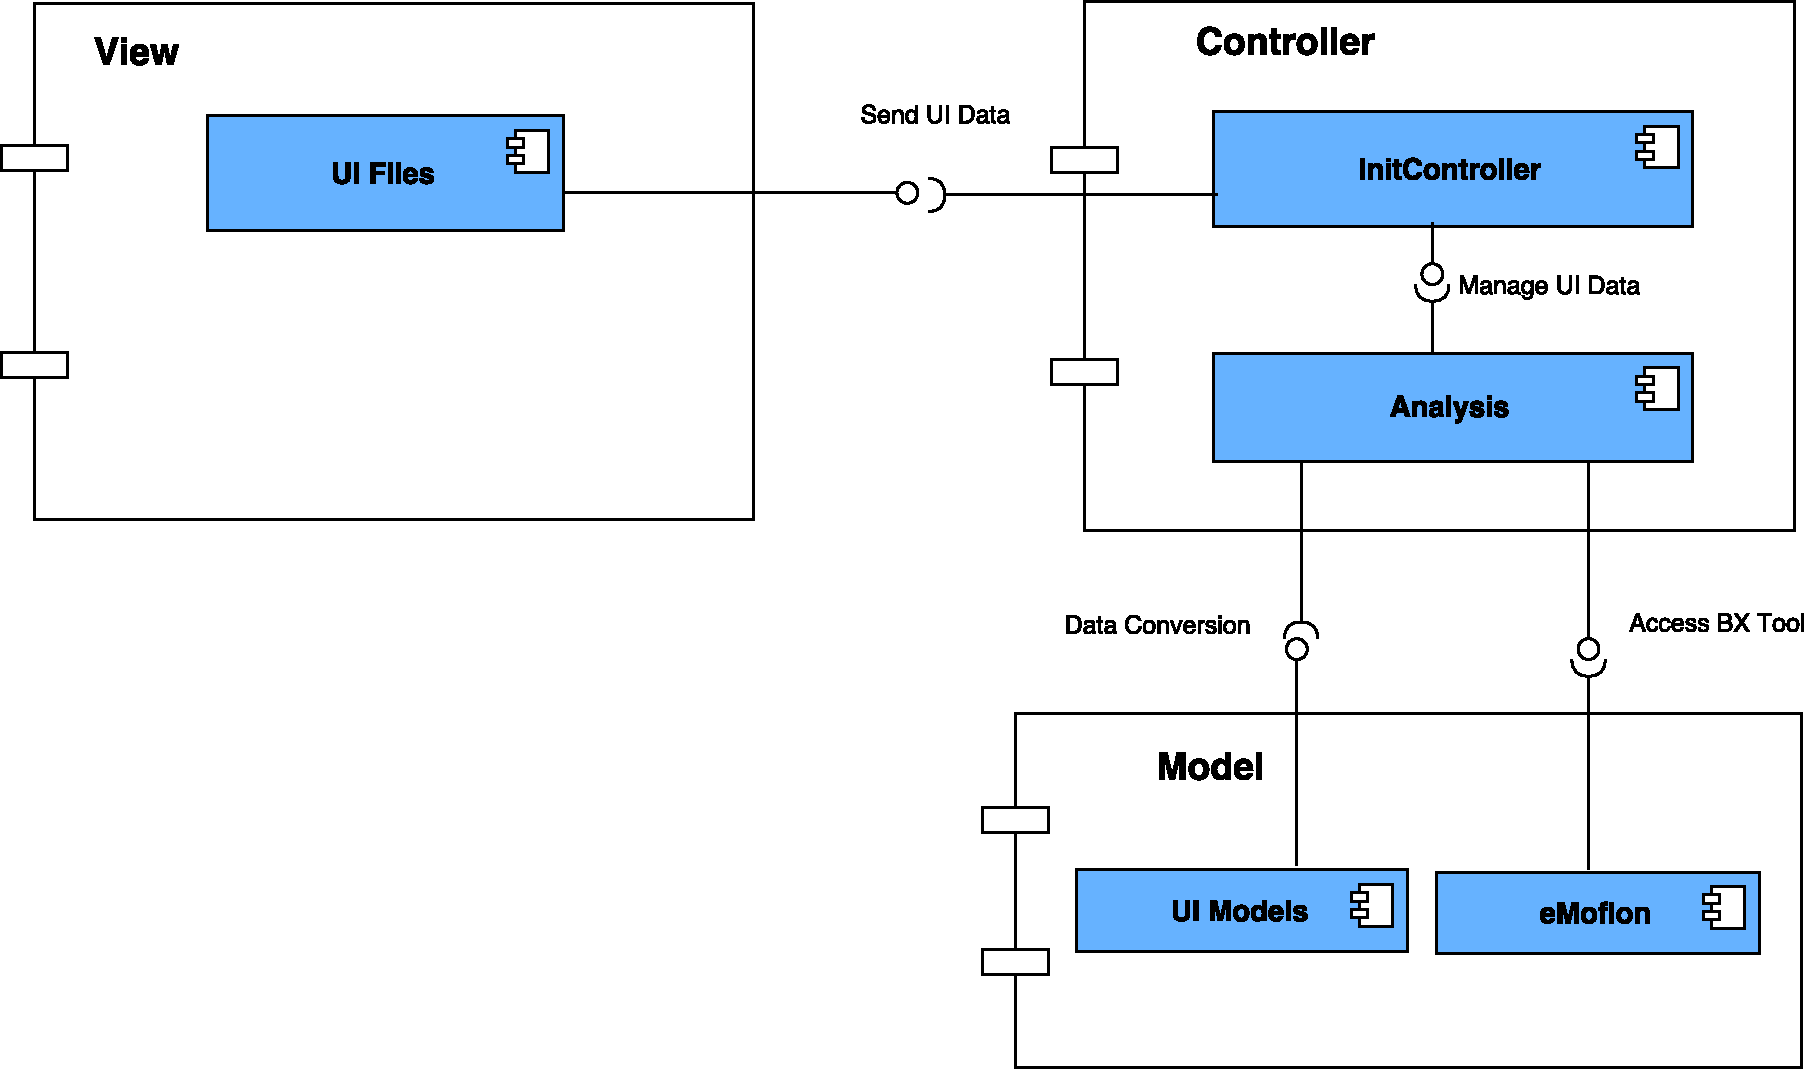
\includegraphics[width=1\textwidth]{figures/Component_Diagram}
	\caption{Component Diagram}
	\label{fig:Component_Diagram}
\end{figure}

I am using Model-View-Controller (MVC) pattern for my application framework. 
On the top, \texttt{View} (Web Browser) component is present which contains a graphical user interface and functionalities that belong to the user. With the changes on \texttt{View} component, data are being provided through interface \texttt{IDoAnalysis} to the \texttt{Controller} component and after the calculations are done, the results are sent back to the \texttt{View} through interface \texttt{IProvideResults}. Both \texttt{View} and \texttt{Controller} resides on the same machine. \texttt{Model} (Bx Tool) component encapsulates and manages the state of all models by communication with the \texttt{Controller} through interface \texttt{IRules}.
\subsubsection{Class Diagram}\label{subsubsec:classes}
\subsubsection{Sequence Diagram}\label{subsubsec:sequence}

\subsection{Core Details}\label{subsec:coredetails}

 




  	\newpage
  	\section{Application}\label{sec:application}
\subsection{Application Walkthrough}\label{subsec:appwalkthrough}



  	\newpage
  	\section{Evaluation}\label{sec:evaluation} 
In this chapter, I am going to evaluate the outcome of my thesis i.e. research and implementation work. 
Figure~\ref{fig:Evaluation_Phases} shows the phases of the entire evaluation process. Section \ref{subsec:goals} describes the research and case study phase. Section \ref{subsec:designmethod} illustrates the evaluation design method that I have used for conducting the experiment. This is then followed by a brief description of the planning phase in Section \ref{subsec:planning}. Afterward, Section \ref{subsec:investigationgoals} deals with the formulas to investigate the goals of the evaluation process. Then, Section \ref{subsec:execution} describes the preparation and test execution phase in detail. Section \ref{subsec:threats&mitigation} explains the associated threats with the evaluation process and their mitigation criteria. At last, Section \ref{subsec:results} discusses the result generated from the gathered data. 

The aim of this chapter is as follows: 

\textbf{"Analyse the outcome of the usage of an interactive demonstrator for the purpose of evaluation with respect to the user from the point of view of the researcher in the context of spreading the basic concepts of bidirectional transformation (bx) and making them understandable and accessible."}

\subsection{Goals}\label{subsec:goals}  
In any research, there could be many cases and each case could focus on a number of different research questions, each of which leads to a different direction in developing solution strategies~\cite{semethods}. Hence, for any evaluation process, most important thing are selecting cases that are most relevant to the research and narrowing down the research questions only associated with the exact problems in hand. 

\begin{figure}
	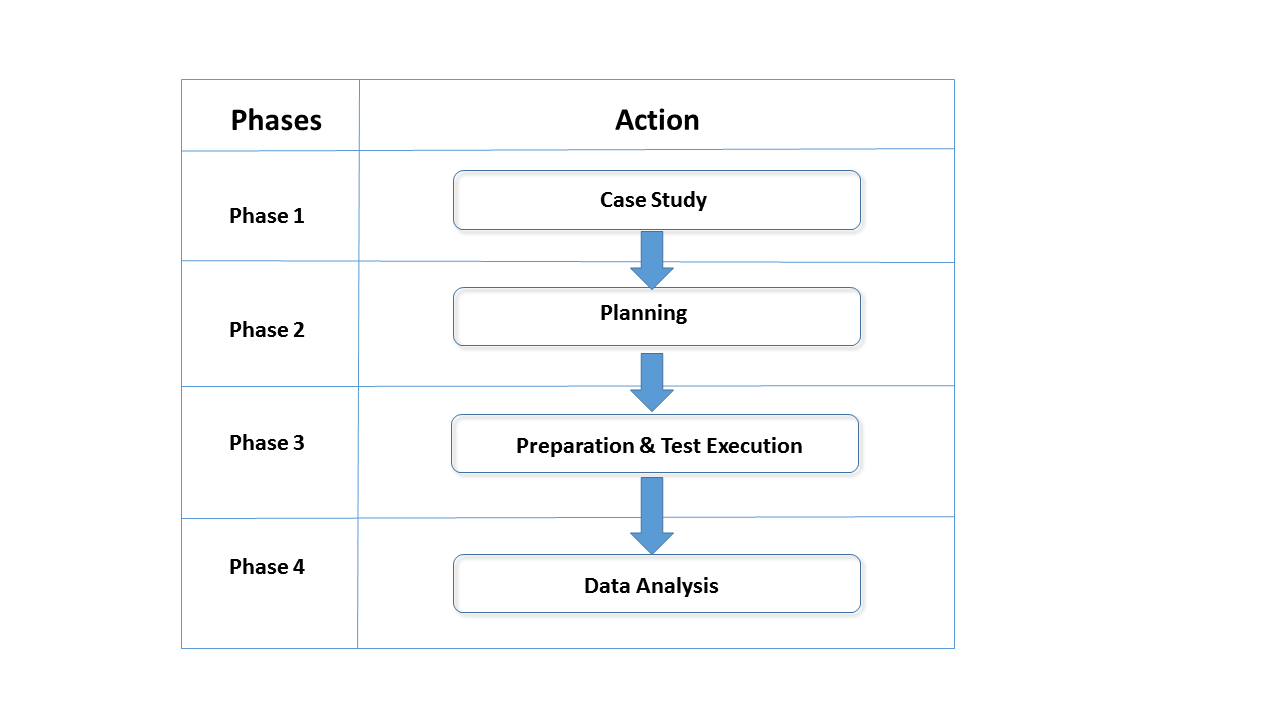
\includegraphics[width=1\textwidth]{figures/Evaluation_Phases}
	\caption{Evaluation Phases}
	\label{fig:Evaluation_Phases}
\end{figure}

\paragraph{Research Questions}
Our experience based on teaching and cooperation with industry has led us to suspect that people often draw their intuition for desired synchronization behavior directly from the special case of bijections.
This can be problematic and leads to statements such as: ``Why do I need a \emph{bidirectional} transformation language if the transformation at hand is not \emph{bijective}?''
Ironically, bidirectional transformation languages are often especially helpful when a transformation is \emph{not} bijective. As a sub-question of the research question \textbf{RQ 3} described earlier in Section \ref{subsec:contribution}, I propose to investigate if such misconceptions are really widespread or not:

\begin{description}
	\item[RQ 3.1:] Do people tend to derive their (in general wrong) intuition for synchronization scenarios from the special case of bijections?
\end{description}

To impart and train a more general intuition for synchronization scenarios I have implemented \texttt{Demon-BX}, an online demonstrator for bidirectional transformations, as a platform for easily creating synchronization scenarios to help achieve corresponding learning goals.
As a proof-of-concept, I have formulated five concrete learning goals and designed corresponding scenarios based on a simple example. We believe (i) that example-based demonstrators are an effective way of achieving my (and similar) learning goals, and (ii) that a demonstrator is only useful in combination with carefully designed scenarios. As a sub-question of the research question \textbf{RQ 4} described earlier in Section \ref{subsec:contribution}, I propose to investigate these conjectures with the following two research questions: 

\begin{description}
	\item[RQ 4.1:] Does demon-bx support achieving corresponding learning goals?
	\item[RQ 4.2:] How much does this support depend on the scenarios?  Would just playing with the demonstrator and the example already have an equal or comparable (positive) effect?
\end{description}

\paragraph{Purpose}
The purpose of the experiment is to evaluate whether it is possible to teach and enhance the understanding of the basic concepts of bx through the demonstrator.

\paragraph{Perspective}
The perspective is from the point of view of the researcher, i.e. the researcher would like to know if the usage of the demonstrator enhances the understanding of bx concepts of a user.

\paragraph{Context}
This experiment is on a bx tool demonstrator which falls under an educational environment and specifically under computer science branch. Hence, this experiment is mainly designed for the group of students/teachers/researchers from computer science area with or without prior knowledge of model driven software development field.

\subsection{Design Method}\label{subsec:designmethod} 
To investigate my research questions, I have used the Pretest-Posttest design method~\cite{analysisprepostdesigns}, a paired data analysis method in which the same experimental object is measured on some variables on two different occasions under different testing conditions. Here, I am using an extension of the Pretest-Posttest design method, called Pretest-Posttest control group design~\cite{expandquasiexpdesign}. It is a highly prestigious and one of the most popular research designs in use. The design principle is relatively simple, which involves two groups, a test group and a control group. First, the groups are pre-tested and then the test group is given the treatment. Afterward, both the groups are post-tested and data is collected from both occasions. Then, the analysis is done by comparing pretest and posttest results collected from both the groups as explained in Figure~\ref{fig:PrePost_Test}.

\begin{figure}
	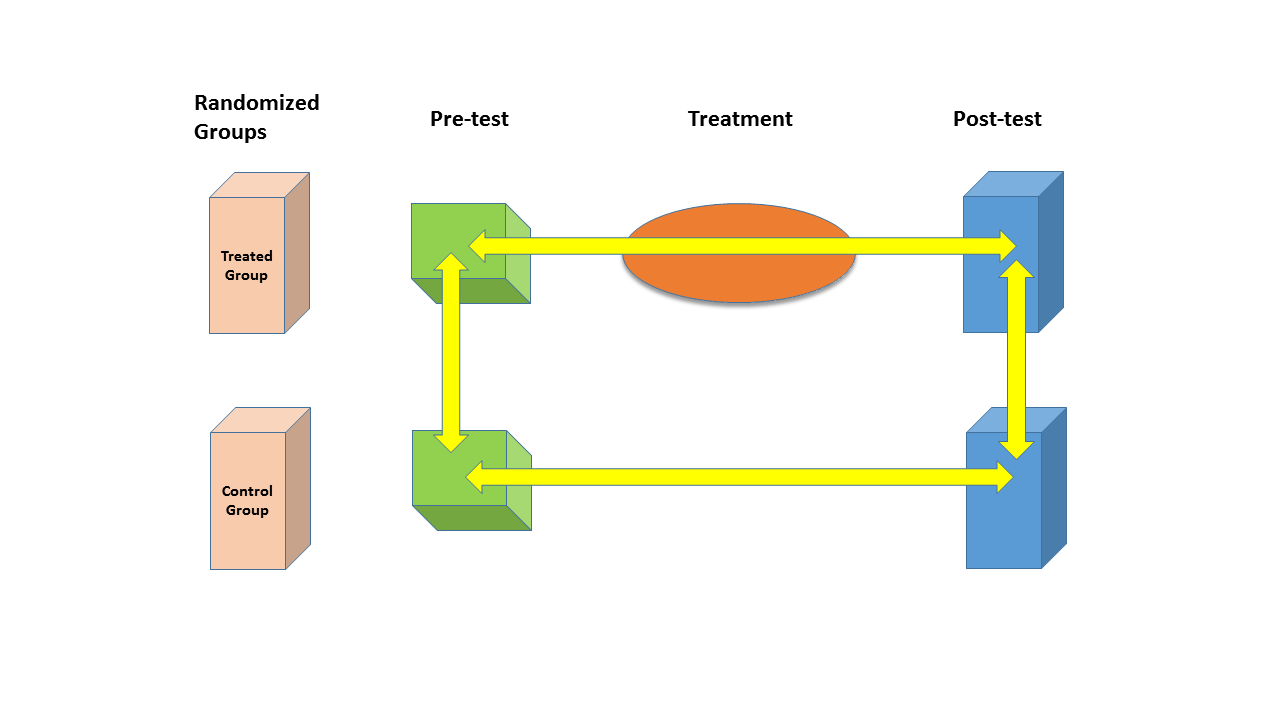
\includegraphics[width=1\textwidth]{figures/PrePost_Test}
	\caption{Pretest-Posttest Control Group Design }
	\label{fig:PrePost_Test}
\end{figure}

Selection of the Pretest-Posttest control group design method for the experiment is driven by the following reasons~\cite{anovapreposttest}:
\begin{itemize}
	\item It provides control over threats to internal validity.
	\item This allows the researchers to collect and compare posttest result from two groups, which give them an idea about the effectiveness of the treatment.
	\item The researcher can see how the groups have performed from pretest to posttest, whether one, both or neither improved over time.
\end{itemize}

In my case, I have designed test questions, one for each learning goal (brief description in Section~ \ref{subsubsec:questions}), to check if a participant has attained the learning goals or not.
We are also interested in the participants' subjective level of certainty for every given answer. 
The experiment is to be conducted as follows:

\begin{enumerate}
	\item All participants are divided randomly into two groups of equal size: the treated group and the control group.
	\item All participants take the pretest (answer all test questions).
	\item Both groups are allowed to use demon-bx for the same amount of time and are provided with an introduction and overview of the concrete example used in the demonstrator.
	The treated group is additionally provided with carefully chosen scenarios to work through, while the control group is not.
	\item When the time is up, all participants take the posttest (answer the same test questions again).
\end{enumerate}

\subsection{Planning}\label{subsec:planning}
This section explains the entire planning phase in detail. In this phase, I have investigated and  finalized all the factors required to evaluate the research questions as well as the execution of the experiment. Following sub-sections describe the factors one by one.

\subsubsection{Participants}\label{subsubsec:participants}
As the context of the experiment is mainly focussed only on the computer science area, it will be conducted on a group of masters' student of computer science branch at Paderborn University. The participants are chosen based on convenience, i.e. the participants are the students taking a similar course.

\subsubsection{Hypotheses}\label{subsubsec:hypotheses}
Formulating hypotheses formally state that what is going to be evaluated in the experiment. I have constructed my hypotheses focussing on the research questions \textbf{RQ 3.1}, \textbf{RQ 4.1}, and  \textbf{RQ 4.2} as described in Section \ref{subsec:goals}. Following are the hypotheses I have chosen to focus in my experiment:\\

\begin{description}
	\item[Operational Hypothesis]
	\item[H$_{OP1}$:] Students derive their (in general wrong) intuition for and expectations of synchronization scenarios from the special case of bijections.
	\item[H$_{OP2}$:] The use of demon-bx has a positive effect on the achievement of corresponding learning goals.\\
	\item[H$_{OP2}$:] The use of demon-bx in combination with suitable scenarios has a positive effect on the achievement of corresponding learning goals.\\
\end{description}

To evaluate the above stated hypotheses, the corresponding null hypotheses are stated below:
\begin{description}
	\item[Null Hypothesis]
	\item[H$_{NU1}$:] Students do not derive their (in general wrong) intuition for the synchronization scenarios.
	\item[H$_{NU2}$:] There is no significant improvement in the learning outcome of the students after using the demon-bx.
	\item[H$_{NU3}$:] There is no significant improvement in the learning outcome of the treated group compared to the control group.

\end{description}

\subsubsection{Experimental Variables}\label{subsubsec:expvariables}
Hypothesis described above helped in deciding the variables related to the experiment. Following paragraphs describe and Table~\ref{tab:Experimental_Variables} summarizes all of them .

\paragraph{Independent Variables} The independent variables, which the experimenter purposely changes during the experiment are listed below:

Does a group get scenarios to work through or not: nominal (yes or no)

\paragraph{Controlled Variables} The controlled variables, which are kept the same throughout the experiment are listed below:

Demonstrator platform: Demon-BX\\
Concrete example: Arranging a Kitchen\\
Group participants are chosen from: \{master students, PhD students, bx researchers, \ldots \}\\
Test questions: 5\\
Learning goals: 5\\
Max. time interval to answer questions: 55 min

\paragraph{Dependent Variables} The dependent variables, which are likely to be changed in response to the independent variable are listed below:

Correctness score of pretest: ordinal\\
Correctness score of posttest: ordinal\\
Level of certainty of pretest:  ordinal\\
Level of certainty of posttest: ordinal

\begin{table}
	\centering	
	\begin{tabular}{|p{4cm}|p{5cm}|p{6cm}|}
		\hline
		\rowcolor[gray]{.8}	
		\textbf{} & \textbf{Name} & \textbf{Possible Values} \\
		\hline
		Independent Variable & Group gets scenarios to work & nominal (yes or no)\\
		\hline
		Controlled Variables & 
		Demonstrator Platform 
		\newline Concrete Example
		\newline Group participants
		\newline Test questions
		\newline Learning goals
		\newline Max. time interval	&
		Demon-BX
		\newline Arranging a Kitchen 
		\newline \{master students, PhD students, \ldots \}
		\newline 5
		\newline 5
		\newline 55 min \\
		\hline	
		Dependent Variables & 
		Correctness score of pretest
		\newline Correctness score of posttest 
		\newline Level of certainty of pretest
		\newline Level of certainty of posttest & 
		ordinal
		\newline ordinal
		\newline ordinal
		\newline ordinal \\
		\hline				
		
	\end{tabular}
	\caption{Experimental Variables}
	\label{tab:Experimental_Variables}
\end{table}

\subsubsection{Learning Goals \& Questions}\label{subsubsec:questions}
To investigate the research questions \textbf{RQ 3} and its sub-question \textbf{RQ 3.1}, I carefully chose five bx concepts to evaluate and imply them as the learning goals (referred to as \textbf{LG} from now on) for the experiment. These concepts are related to the basic fundamentals of bx described as follows:
\begin{description}
	\item[LG 1:] It is possible to avoid/minimize unnecessary information loss in bx. 
	\item[LG 2:] Not all possible changes done in one model can be translated/synchronized into another model.
	\item[LG 3:] Synchronisation is interactive. User interaction (or some other, possibly automated means) can be used to decide between multiple equally consistent results (to handle non-determinism). 
	\item[LG 4:] Undoing changes in one model to revert to a previous state does not necessarily imply that this can be reflected analogously in the other model. 
	\item[LG 5:] Bx frameworks are not always state based but also can be delta based. The actual change performed can have an effect on synchronization results, even if the final result might appear to be exactly the same in both cases. 
\end{description}

To evaluate these learning goals, I prepared five questions. Each question referred to a concept of bx which also corresponds to a learning goal.

The questions are designed to have two sections for answers. One section contains multiple choice answers and the other contains certainty scale ranging from "I just guessed" to "I am certain". Correctness will be decided from the selection of answer in multiple choice section and certainty will be decided from the certainty parameters. Hence, combining the answer and the certainty parameter I can differentiate between \emph{correct answer}, \emph{absolute correct answer}, \emph{wrong answer}, and \emph{absolute wrong answer}.

\subsection{Execution}\label{subsec:execution} 
This section explains the entire experiment execution process in detail along with the preparation steps in the following subsections.

\subsubsection{Preparation }\label{subsubsec:prep}
To handle two separate groups i.e., control and treated and to conduct two separate tests i.e., pre-test and post-test on them, I had to prepare well before the experiment date. 

First, I prepared a two-minute video tutorial explaining some of the basic concepts of bx. Then, I prepared a set of questions  relating each question to one learning goals and put them into two different forms  i.e., pretest and posttest prepared with google forms to make them available online for the sake of easy sharing. Then to investigate the research questions \textbf{RQ 4} and its sub-question \textbf{RQ 4.1}, I prepared the scenarios with the demonstrator to explain the learning goals in a simple way but with a concrete example. Finally, I prepared two different instruction sheets for both the groups explaining the steps they need to follow during the experiment.

\subsubsection{Test Execution}\label{subsubsec:execution}
The experiment was performed on a group of Master students attending a computer science lecture at Paderborn University. They were informed in advance that such experiment will be conducted on a particular date and that their participation in the experiment is completely voluntary with no consequences what so ever. Participants were requested to bring their laptops to the lecture on the day of the experiment.

\paragraph{Confidentiality} The participants were informed regarding the confidentiality and anonymity of data. The purpose of evaluating the tool was stated, but not the hypotheses of the experiment.

\paragraph{Randomization} To perform the experiment, the students were given the instruction sheet prepared earlier for either the control or the treated group randomly while entering the room. The participants were not informed about which group they are in and received suitable and separate instructions for each group.

\paragraph{No Interference} After that, they were asked to sit in two different areas according to their group allotment. The groups were spatially separated so that discussion between groups was almost impossible.

These information sheets had all the appropriate links to the corresponding questionnaires with questions for the pre-test and post-test, demonstrator links with prepared scenarios for the treated group, and a different demonstrator link without scenarios for the control group.

Firstly, all participants went through a two-minute video tutorial to establish basic concepts and notation used in the test questions. Then all participants were asked to take the pre-test. After finishing the pre-test, the students were asked to use the demonstrator links given to them and to work with it. The link given to the control group only had information on how to operate the demonstrator, while the treated group had access to scenarios chosen to support my learning goals. 

After playing with the demonstrator, both groups were asked to take the post-test. Post-test questions were exactly the same as pre-test questions but include some extra questions to get additional qualitative feedback about the demonstrator. The experiment was stopped exactly after 55 minutes.

\subsubsection{Data Validation}\label{subsubsec:datavalidation}
Data was collected from 40 students. I stopped taking responses on Google forms i.e. pre-test and post-test forms from students exactly after 55 minutes. After the experiment, I checked the data entered by students in both the forms. Data from one student was removed, due to the fact that the data was regarded as invalid as the student could not finish both the test in the given time limit.

Hence, after removing one student out of the 40, I had data from 39 students for statistical analysis and interpretation of the results.

Finally, based on unique identifiers (identifying the group and participant uniquely) derived for each participant, answers from pre-test and post-test were evaluated to get the results. 

\subsection{Threats to Validity and Mitigation}\label{subsec:threats&mitigation}
A good research work depends highly on its validity and quality of work involved and results. So, it is very important to consider, analyze and mitigate the validity threats to the research work and the results. In my evaluation, I have focused on the validity analysis and threats given by Wohlin et al~\cite{expinse} and further explained by Feldt et al~\cite{validitythreatsinse}. Wohlin et al discuss four main types of validity threats: internal, external, construct and conclusion. 

This section describes all the threats that are associated with the entire evaluation process i.e., planning, preparation, and execution in the following subsections.
 
\subsubsection{Internal Validity}\label{subsubsec:internalvalidity}
\emph{Did the treatment/change I introduced cause the effect on the outcome? Can other factors also have had an effect?}

\medskip
\noindent To measure improvement I am forced to perform arithmetic with ordinal values.
This might be problematic as the difficulty of the test questions might not be equal (although I have tried to ensure this). If, for example, one of the test questions is much more difficult than all the rest, then subtracting test scores and comparing improvements between groups is questionable. Hence to make the questions/concepts more understandable, I have provided some explanations in the post-test as a video tutorial showing the relation between the abstract example and a concrete example.

\subsubsection{External Validity}\label{subsubsec:externalvalidity}
\emph{Is the cause and effect relationship I have shown valid in other situations?}

\medskip
\noindent Our results are only valid for the choice of control variables.
This can be problematic as, for example, my test questions might not actually be suitable for checking if my learning goals have been reached.

\subsubsection{Construct Validity}\label{subsubsec:constructvalidity}
\emph{Do the groups involved in the experiment equally balanced to have a positive effect on the outcome I measure?}

\medskip
\noindent It might be possible that students of equal caliber are sitting together or might have a discussion between the test to have a negetive effect on the results. Hence to avoid that, I have randomly selected students for control and treated group by giving them instruction sheets randomly while entering the class and making them sit in two separate groups apart from each other.

\subsubsection{Conclusion Validity}\label{subsubsec:conclusionvalidity}
\emph{Does the treatment/change I introduced have a statistically significant effect on the outcome I measure? Can I draw conclusions based on the data?}
	
\medskip
\noindent A problem could be that participants just guess the answers wildly. So it might possible that the data could be faked or incorrect due to mistakes. To avoid faking of data and to add more authenticity to the experiment, I have added certainty values for each question so that I will get to know whether the participant is just guessing the answer or certain about it. Also, I have scrambled the order of the scenarios given to the treated group to play with and the questions asked so that participants will not get a clue about the relation between them.

\subsection{Data Analysis, Results, and Discussion}\label{subsec:results}
To get the results for my experiment, I have investigated on each hypothesis with the data collected separately. Analysis of the data, descriptive statistics are used to visualize the data collected and described in the following subsections.

\subsubsection{Analyzing Hypothesis 1}\label{subsubsec:hypothesis1}
Hypothesis 1 i.e., \textbf{H$_{OP1}$} and \textbf{H$_{NU1}$} is designed to investigate research question \textbf{RQ 3.1}.
\paragraph{Formula} Data for \textbf{RQ 3.1} can be collected from all pretest results i.e., combining the pretest results from both control and treated group. As five questions were asked, result can be calculated for each question from the pretest data. 

Calculation of the result for each question involves the correctness and certainty of the answers given by the students.
For ith Question \textit{Q$_{i}$},

\textit{CO$_{pre(i)}$} $\epsilon$ \{-1, 1\}, correctness of the answer to the ith pretest question is either right (1) or wrong (-1).

\textit{CE$_{pre(i)}$} $\epsilon$ [0, 1], certainty of the answer to the ith pretest question is between 0 ("I just guessed") to 1 ("I am certain").

\textit{RES$_{pre(i)}$} := \textit{CO$_{pre(i)}$} * \textit{CE$_{pre(i)}$} $\epsilon$ [-1,  1], result for the ith pretest question is between -1 to 1.

For the final calculation, following result will be considered:\\
\textit{R$_{pre(i)}$}:= Set containing all the \textit{RES$_{pre(i)}$} calculated from the answers to the ith pretest question.

Null Hypothesis, {H$_{NU1}$}: Mean (\textit{R$_{pre(i)}$}) <= 0

Operational Hypothesis, {H$_{OP1}$}: Mean (\textit{R$_{pre(i)}$}) > 0

\paragraph{Data Analysis}
\paragraph{Discussion}

\subsubsection{Analyzing Hypothesis 2}\label{subsubsec:hypothesis2}
Hypothesis 2 i.e., \textbf{H$_{OP2}$} and \textbf{H$_{NU2}$} is designed to investigate research question \textbf{RQ 4.1}.

\paragraph{Formula}
Data for \textbf{RQ 4.1} can be collected from all pretest and posttest results i.e., combining the pretest results from both control and treated group and combining the posttest results from both control and treated group. As five questions were asked, result can be calculated for each question from the pretest and posttest data. 

Calculation of the result for each question involves calculation of improvement in correctness and certainty of the answers given by the students in posttest than pretest.
For ith Question \textit{Q$_{i}$},

\textit{CO$_{pre(i)}$} $\epsilon$ \{-1, 1\}, correctness of the answer to the ith pretest question is either right (1) or wrong (-1).

\textit{CE$_{pre(i)}$} $\epsilon$ [0, 1], certainty of the answer to the ith pretest question is between 0 ("I just guessed") to 1 ("I am certain").

\textit{RES$_{pre(i)}$} := \textit{CO$_{pre(i)}$} * \textit{CE$_{pre(i)}$} $\epsilon$ [-1,  1], result for the ith pretest question is between -1 to 1.

\textit{CO$_{post(i)}$} $\epsilon$ \{-1, 1\}, correctness of the answer to the ith posttest question is either right (1) or wrong (-1).

\textit{CE$_{post(i)}$} $\epsilon$ [0, 1], certainty of the answer to the ith posttest question is between 0 ("I just guessed") to 1 ("I am certain").

\textit{RES$_{post(i)}$} := \textit{CO$_{post(i)}$} * \textit{CE$_{post(i)}$} $\epsilon$ [-1,  1], result for the ith posttest question is between -1 to 1.

\textit{IMP$_{(i)}$} := (\textit{RES$_{post(i)}$} - \textit{RES$_{pre(i)}$})/2 $\epsilon$ [-1,  1], improvement for the ith question from pretest to posttest is between -1 to 1.

For the final calculation, following result will be considered:\\
\textit{I$_{(i)}$}:= Set containing all the \textit{IMP$_{(i)}$} calculated from the answers.

Null Hypothesis, {H$_{NU1}$}: Mean (\textit{I$_{(i)}$}) <= 0

Operational Hypothesis, {H$_{OP1}$}: Mean (\textit{I$_{(i)}$}) > 0

\paragraph{Data Analysis}
\paragraph{Discussion}
\subsubsection{Analyzing Hypothesis 3}\label{subsubsec:hypothesis3}
Hypothesis 3 i.e., \textbf{H$_{OP3}$} and \textbf{H$_{NU3}$} is designed to investigate research question \textbf{RQ 4.2}.

\paragraph{Formula}
Data for \textbf{RQ 4.2} can be collected from all pretest and posttest results separately from control and treated group. As five questions were asked, result can be calculated for each question from the pretest and posttest data separately for control and treated group. 

Calculation of the result for each question involves calculation of improvement in correctness and certainty of the answers given by the students in posttest than pretest separately for control and treated group.
For ith Question \textit{Q$_{i}$},

Parameters used in the below formulas e.g., \textit{RES$_{post(ci)}$}, \textit{RES$_{pre(ci)}$}, \textit{RES$_{post(ti)}$}, \textit{RES$_{pre(ti)}$} are calculated similar to the formulas as described in Section \ref{subsubsec:hypothesis2} but separately for control and treated group.

\textit{IMP$_{(ci)}$} := (\textit{RES$_{post(ci)}$} - \textit{RES$_{pre(ci)}$})/2 $\epsilon$ [-1,  1], improvement for the control group for the ith question from pretest to posttest is between -1 to 1.

\textit{IMP$_{(ti)}$} := (\textit{RES$_{post(ti)}$} - \textit{RES$_{pre(ti)}$})/2 $\epsilon$ [-1,  1], improvement for the treated group for the ith question from pretest to posttest is between -1 to 1.

For the final calculation, following result will be considered:\\
\textit{I$_{(ci)}$}:= Set containing all the \textit{IMP$_{(ci)}$} calculated from the answers of the control group.

\textit{I$_{(ti)}$}:= Set containing all the \textit{IMP$_{(ti)}$} calculated from the answers of the treated group.

Null Hypothesis, {H$_{NU1}$}: Mean (\textit{I$_{(ci)}$})  - Mean (\textit{I$_{(ti)}$}) < 0

Operational Hypothesis, {H$_{OP1}$}: Mean (\textit{I$_{(ci)}$})  - Mean (\textit{I$_{(ti)}$}) > 0


\paragraph{Data Analysis}
\paragraph{Discussion}
  	\newpage
  	\section{Summary and Future Work}\label{sec:summary}
In this chapter, I am going to conclude the entire work done in this thesis. Section \ref{subsec:conclusion} summarizes the work done and explained in the previous chapters, and  Section \ref{subsec:futurework} discusses some future enhancements that can be applied to the current work.

\subsection{Conclusion}\label{subsec:conclusion}
With this thesis, I tried to solve the problem of a missing platform for teaching bx concepts by designing and implementing an interactive demonstrator built on the top of a bx tool. The principal task was to design an application framework with an interface to communicate with bx tools and demonstrate their features on an interactive user interface.

In the process of solving the problems stated earlier, the following were my contributions:
\begin{enumerate}
	\item {\textit{Analysis and design of the application framework}: I have designed a working, fully functional application framework based on MVC pattern by extending the interface designed for accessing bx tools by Anjorin et al. \cite{benchmarx-reload} for implementing a bx tool demonstrator along with an interactive user interface. This framework can be used to implement a demonstrator encapsulating bx tools with concrete examples. Also, it is easy to add additional scenarios to teach bx related concepts, fairly easy to add different versions of the rules used, fairly easy to swap the bx tool, and more or less easy to implement a new example as long as it can work with the user interface.}
    \item {\textit{Concrete implementation of the demonstrator}: After analyzing the existing work on bx and their related problems as described in Section \ref{sec:relatedwork}, I designed the requirements of my demonstrator to overcome these problems. Afterward, I have implemented a fully functional online demonstrator based on the application framework designed earlier and checked its feasibility and validity. My demonstrator i.e., Demon-BX satisfies all the requirements listed in Section \ref{sec:requirements} and hence overcomes the identified problems with the existing demonstrator platform for bx. This demonstrator is based on a bx tool i.e., eMoflon and a concrete example leveraging the functionalities of the bx tool and explaining some basic bx concepts.}
    \item {\textit{Evaluation of the demonstrator}: After the implementation, I have evaluated the demonstrator based on the research method called Pretest-Posttest control group design~\cite{expandquasiexpdesign} to check its effectiveness and impact. This experiment was driven by three hypotheses and a few experimental variables i.e., dependent, independent, and controlled. A well-designed experiment was performed with two different groups of participants, data were collected and analyzed to measure the outcome.}
	
\end{enumerate}

With the above contributions, I was able to build a web platform for a bx tool which is easily accessible to a widespread audience. My demonstrator helps to demonstrate the features of the bx tool, eMoflon along with a few bx concepts. A user can easily try my demonstrator in no time with a few mouse clicks and avoid the complex and time-consuming process which is required in the case of virtual machines, tutorials \& handbooks to get a bx tool running. 

With these findings, I was able to answer the following research questions with respect to the requirements:
\begin{table}[h]
	\begin{tabular}{|p{5cm}|p{9.5cm}|}
		\hline
		\rowcolor[gray]{.8}	
		\textbf{Research Questions} & \textbf{Solutions}\\
		\hline
		\textbf{RQ1 -} What are the core requirements for implementing a successful bx demonstrator? &
		From the work of my thesis, I feel that the most important requirements for implementing a successful bx demonstrator are the functional \& non-functional behaviors as described in Section \ref{sec:requirements}. For example that the user should able to initiate the synchronization process in both directions, the user should able to manipulate the models before synchronization, the example should be simple and fun to play with, the GUI should be interactive, zero setup time for the demonstrator, there is some interaction involved and perhaps decision making while playing with the example, the demonstrator should be accessible worldwide and platform independent, etc. \\
		\hline
		\textbf{RQ2 -} To what extent is such a bx demonstrator reusable? &
		A few dimensions involved with the implementation of a bx demonstrator are (i) addition of different synchronization rules, (ii) visualization of different examples, and (iii) the ability to demonstrate the features of different bx tools. From the implementation work of my demonstrator, I can say that my application framework along with the extended interface for accessing the bx tools can be reused/extended to realize these dimensions. It is fairly easy to add different versions of the rules used, fairly easy to swap the bx tool, and more or less easy to implement a new example as long as it can work with the UI.\\
		\hline
		\textbf{RQ3 -} Is there a need to teach the concepts of bx through a demonstrator? &
		It is evident from the outcome of the hypothesis H$_{OP1}$ (which corresponds to the research question \textbf{RQ3.1}) that the students derive their (in general wrong) intuition for and expectations of synchronization scenarios from the special case of bijections. Hence, there is indeed a need to teach correct expectations for synchronization scenarios and a demonstrator can be potentially very useful in spreading bx concepts.\\
		\hline				
	\end{tabular}
	\label{tab:Solutions_ResearchQuestions}
\end{table}

\begin{table}
	\begin{tabular}{|p{5cm}|p{9.5cm}|}
		\hline	
		\textbf{RQ4 -} Does an interactive GUI helps a user to increase his/her understanding related to bx concepts? &
		To teach bx related concepts through the demonstrator, I have carefully designed the corresponding scenarios by combining them with different parts of the implemented example  and allowed the user to play with it in order to learn the concepts. However, this is indeed quite challenging. It is evident from the outcome of the hypotheses H$_{OP2}$ and H$_{OP3}$ (which corresponds to the research question \textbf{RQ4.1} and \textbf{RQ4.2} respectively) that without carefully designed scenarios there is no guarantee that the learning goals (\textbf{LG}s) are addressed and there might even be negative learning.  With scenarios, the situation is a bit better but I was not able to conclude this with statistical significance.\\
		\hline			
	\end{tabular}
	\caption{Solutions to the Research Questions}
	\label{tab:Solutions_ResearchQuestions}
\end{table}

\subsection{Future Work}\label{subsec:futurework}
In this thesis, I have designed an application framework for the bx tool demonstrator, implemented the demonstrator based on a concrete example, and further evaluated the demonstrator to check its effectiveness in order to teach bx concepts to a widespread audience to the best of my knowledge and belief. However, a few other features that were out-of-scope for this thesis can be added to the current work done. In the following paragraphs, I discuss some enhancements that can be applied to my work in the future. 
\paragraph{New Rules}
My current implementation of the eMoflon tool is based on two meta models and five transformation rules. However, it will be interesting to add a few more transformation rules for the existing meta-models. It will surely enhance the interactivity of the demonstrator and also test the capability of UI on handling new rules.

\paragraph{New Examples} I have implemented one example i.e., \textit{Planning a Kitchen} in the demonstrator. However, it would be fascinating to see the implementation of a few more examples on the same or different UI platform but on the top of the same application framework. Some new examples will definitely test and verify the robustness of the application framework as well as the features of the eMoflon tool further.

\paragraph{Another BX Tool}
Demon-BX is implemented encapsulating the features of the bx tool \texttt{eMoflon}. However, to test the application framework and the interface built for communicating with bx tools, implementation of another bx tool can be researched and added to the current work. 

\paragraph{BX Tool as a Webservice}
In the current implementation of Demon-BX, the \texttt{Model} component in the application framework is built as a Java project. Due to a Java project, it has a very thin binding with the \texttt{Controller} component. Any changes in model component related to class name, method name and their accessibility will affect the implementation of the \texttt{Adapter} class. Hence, to remove this dependency, the model component can be designed and implemented as a web service. After that, the model can be seen as a plug-in component communicating through JSON/XML data, which completely removes its dependency on the controller component. Hence, any researcher can implement the synchronization with their tool and use the web service.

\paragraph{New Experiment}
As per the research method Pretest-Posttest control group design~\cite{expandquasiexpdesign}, only treated group should be exposed to the treatment which the researcher wants to test. However, in my experiment, the control group was given the demonstrator without any scenarios and then asked to answer the posttest question. This might affect the final output as somehow control group was exposed to the demonstrator environment and can cause the same effect what treated group experienced with scenarios. Hence, a new experiment can be done by showing the control group only a video about bx concepts in relation with a concrete example instead of exposing them to the demonstrator environment.





    \clearpage
    
    \section{Appendix}\label{sec:Appendix}

\paragraph{Servlet Lifecycle}
Figure~\ref{fig:Server_Servlet} describes the complete lifecycle of a servlet w.r.t. a web server and a web container. The lifecycle steps are described as follows \cite{servlet}:

\begin{figure}[h]
	\centering
	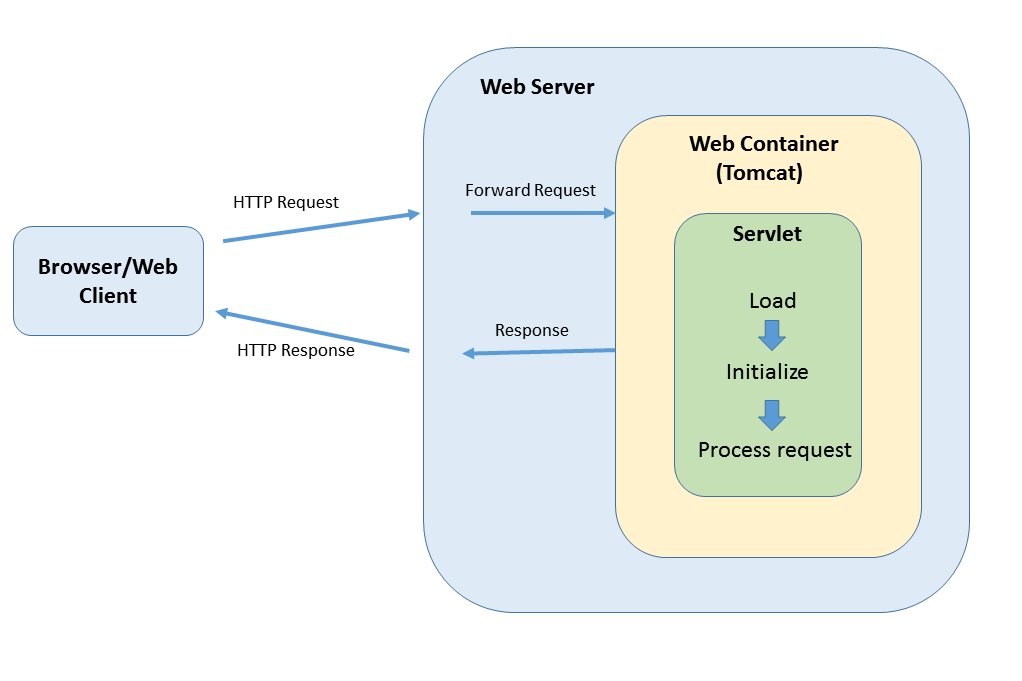
\includegraphics[width=1\textwidth]{figures/Server_Servlet}
	\caption{Servlet Lifecycle}
	\label{fig:Server_Servlet}
\end{figure}

\begin{enumerate}
	\item {The web server receives the \texttt{HTTP request} from the client interacting through a browser. After accepting the request, web server forwards the request to the web container i.e., Tomcat.}
	\item {Web container sends the request to the \texttt{Servlet class}. If an instance of the servlet does not exist, the web container loads the servlet class then creates an instance of the servlet class and initializes the servlet instance by calling the \texttt{init} method.}
	\item {After that, web container invokes the \texttt{service} methods (normally HTTP methods i.e., \texttt{get} , \texttt{post} , \texttt{put} , \texttt{delete}) of the servlet class by passing the request and response objects and the actual processing of the request is done and the response is generated.}
	\item {Web container sends the response to the web server. Afterward, web server creates the HTTP response and send it back to the client.}
\end{enumerate}

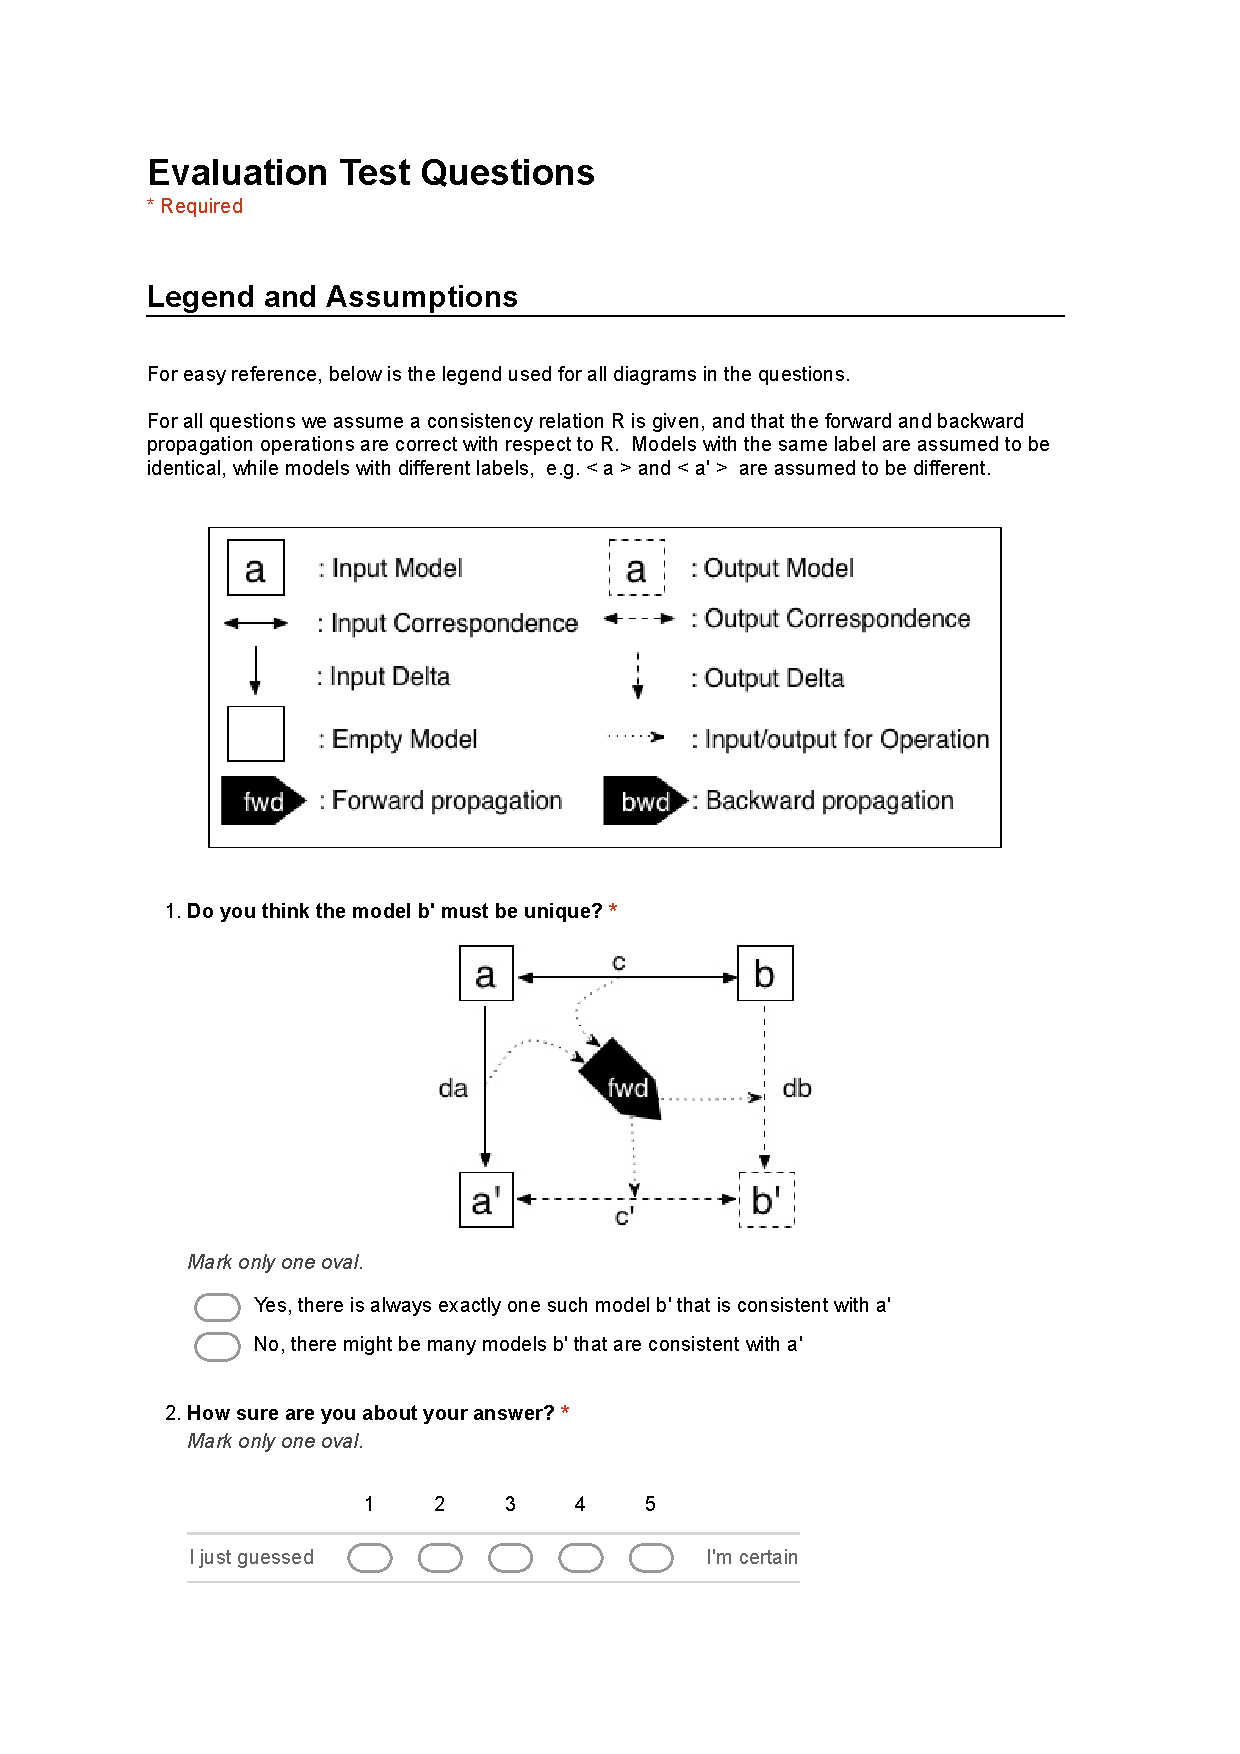
\includepdf[pages={1-5}]{figures/Evaluation_TestQuestions}

\paragraph{Transformation Rules} In this paragraph, I have described all the transformation rules implemented with eMoflon tool for the source and target models. Source models consist of a single \texttt{Grid}, with \texttt{Groups} that can occupy multiple \texttt{Blocks}. \texttt{Blocks} are additionally connected with all their neighbouring blocks. Target models consist of a single \texttt{Kitchen} with \texttt{ItemSockets} as placeholders for exactly one \texttt{Item}, i.e., sink, fridge, table etc.

1. \textit{Kitchen\_to\_Grid: }  Figure~\ref{fig:TR_Kitchen_to_Grid} describes that if you create a \texttt{Grid} in the source, then you should create a corresponding \texttt{Kitchen} in the target.

\begin{figure}[h]
	\centering
	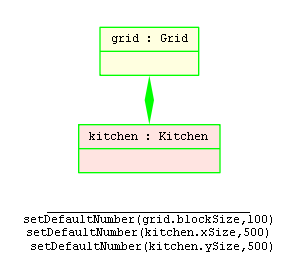
\includegraphics[width=0.7\textwidth]{figures/TR_Kitchen_to_Grid}
	\caption{Transformation Rule: Kitchen\_to\_Grid}
	\label{fig:TR_Kitchen_to_Grid}
\end{figure}

2. \textit{ItemSocket\_to\_Group: } Figure~\ref{fig:TR_ItemSocket_to_Group} describes that if you add a new \texttt{Group} to the grid, then you should add an \texttt{ItemSocket} (a placeholder for items) to the kitchen.

\begin{figure}[h]
	\centering
	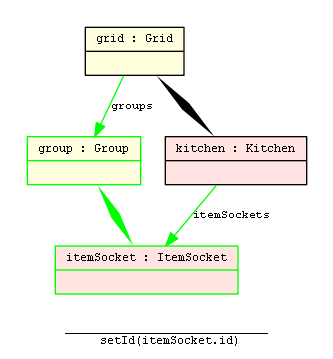
\includegraphics[width=0.5\textwidth]{figures/TR_ItemSocket_to_Group}
	\caption{Transformation Rule: ItemSocket\_to\_Group}
	\label{fig:TR_ItemSocket_to_Group}
\end{figure}

3. \textit{Create\_a\_Sink: } Figure~\ref{fig:TR_Create_a_Sink} describes that a \texttt{Sink} must be created on the western wall and occupies two horizontal blocks.

\begin{figure}[h]
	\centering
	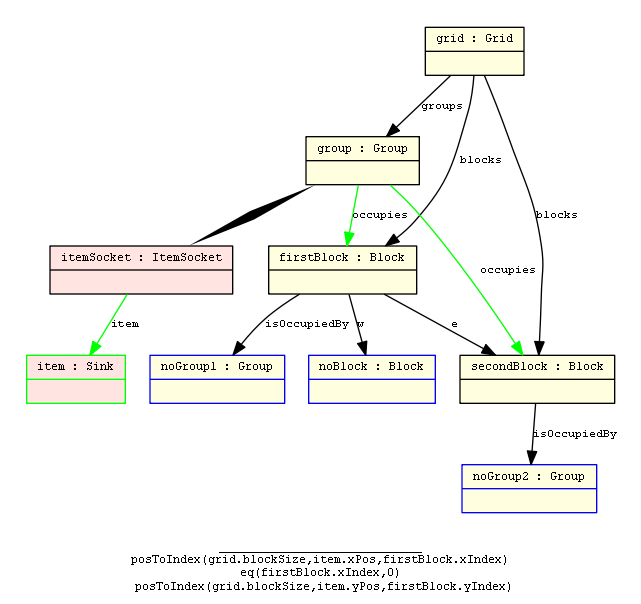
\includegraphics[width=0.7\textwidth]{figures/TR_Create_a_Sink}
	\caption{Transformation Rule: Create\_a\_Sink}
	\label{fig:TR_Create_a_Sink}
\end{figure}

4. \textit{Create\_a\_Fridge: } Figure~\ref{fig:TR_Create_a_Fridge} describes that a \texttt{Fridge} must be created on the northern wall and occupies two vertical blocks.

\begin{figure}[h]
	\centering
	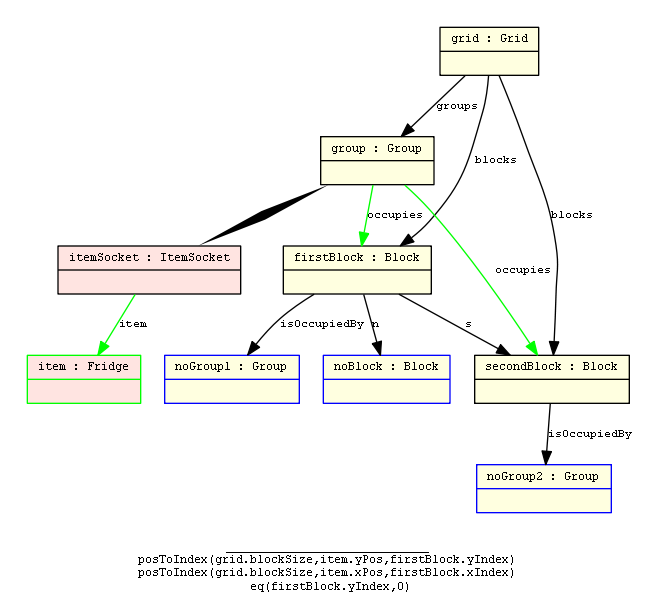
\includegraphics[width=0.8\textwidth]{figures/TR_Create_a_Fridge}
	\caption{Transformation Rule: Create\_a\_Fridge}
	\label{fig:TR_Create_a_Fridge}
\end{figure}

5. \textit{Create\_a\_Horizontal\_Table: } Figure~\ref{fig:TR_Create_a_Horizontal_Table} describes that if you create a \texttt{Horizontal Table}, then its group should be placed on two blocks horizontally.

\begin{figure}[h]
	\centering
	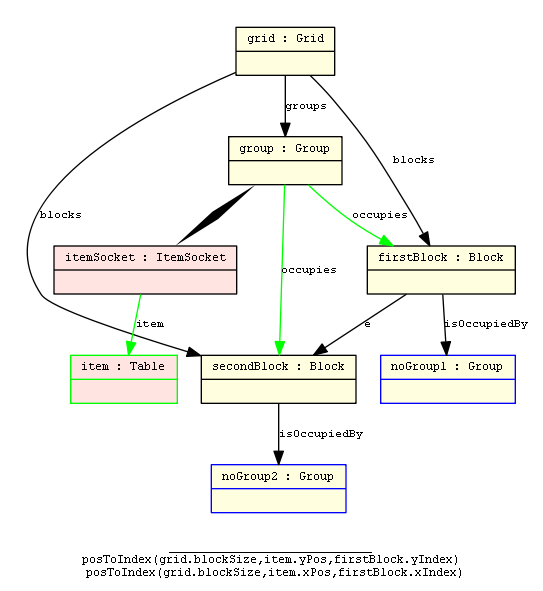
\includegraphics[width=0.8\textwidth]{figures/TR_Create_a_Horizontal_Table}
	\caption{Transformation Rule: Create\_a\_Horizontal\_Table}
	\label{fig:TR_Create_a_Horizontal_Table}
\end{figure}

6. \textit{Create\_a\_Vertical\_Table: } Figure~\ref{fig:TR_Create_a_Vertical_Table} describes that if you create a \texttt{Vertical Table}, then its group should be placed on two blocks vertically.

\begin{figure}[h]
	\centering
	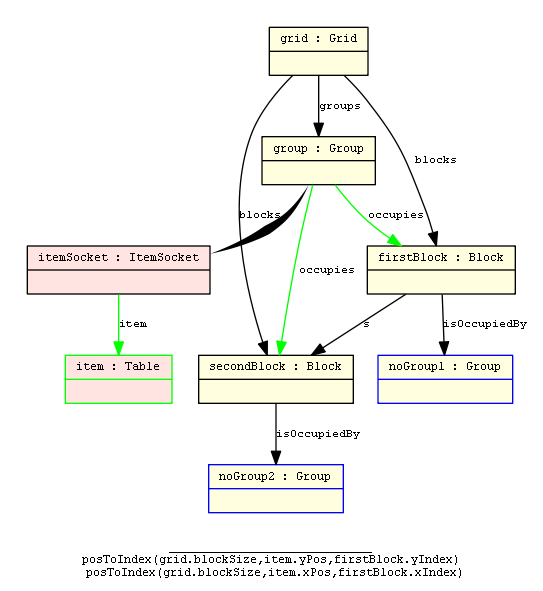
\includegraphics[width=0.8\textwidth]{figures/TR_Create_a_Vertical_Table}
	\caption{Transformation Rule: Create\_a\_Vertical\_Table}
	\label{fig:TR_Create_a_Vertical_Table}
\end{figure}

    \clearpage
  	\listoffigures
  	\clearpage
  	\listoftables
  	\clearpage
  	
  	\begin{thebibliography}{1}
	
	\bibitem{bx-grace} K. Czarnecki, J. N. Foster, Z. Hu, R. L\"ammel, A. Sch\"urr, and J. F. Terwilliger,  {\em Bidirectional Transformations: A Cross-Discipline Perspective}, GRACE International Meeting , Shonan, Japan, 2008.
	
	\bibitem{bx-dagstuhl} Z. Hu, A. Sch\"urr, P. Stevens, and J. Terwilliger,  {\em Dagstuhl Seminar} \#11031 on Bidirectional Transformations "bx", Dagstuhl Reports, Vol. 1, Issue 1, pages 42-67, January 16-21 , 2011.
	
	\bibitem{bx-theoryandappl} J. Gibbons, R. F. Paige, A. Sch\"urr, J. F. Terwilliger and J. Weber, {\em Bi-directional transformations (bx) - Theory and Applications Across Disciplines}, [Online]. Available:  https://www.birs.ca/workshops/2013/13w5115/report13w5115.pdf.
	
	\bibitem{benchmark-BX} R. Oppermann and P. Robrecht, {\em Benchmarks for Bidirectional Transformations.} Seminar Maintaining Consistency in Model-Driven Engineering: Challenges and Techniques, University of Paderborn: Summer Term 2016.
	
	\bibitem{benchmarx} A. Anjorin, A. Cunha, H. Giese, F. Hermann, A. Rensink, and A. Sch\"urr, {\em Benchmarx}. In K. S. Candan, S. Amer-Yahia, N. Schweikardt, V. Christophides, and V. Leroy, editors, Proceedings of the Workshops of the EDBT/ICDT 2014 Joint Conference (EDBT/ICDT 2014), CEUR Workshop Proceedings, pages 82-86. CEUR-WS.org, 2014.
		
	\bibitem{benchmarx-reload} A. Anjorin, Z. Diskin, F. Jouault, Hsiang-Shang Ko, E. Leblebici, and B. Westfechtel, {\em Benchmarx Reloaded: A Practical Benchmark Framework for Bidirectional Transformations}. In R. Eramo, M. Johnson (eds.): Proceedings of the Sixth International Workshop on Bidirectional Transformations (Bx 2017),
	Uppsala, Sweden, April 29, 2017, published at http://ceur-ws.org.
	
	\bibitem{tgg} A. Sch\"urr. {\em Specification of graph translators with triple graph grammars.} In E. W. Mayr, G. Schmidt, and G. Tinhofer, editors, {\em Graph-Theoretic
	Concepts in Computer Science, 20th International Workshop, WG 94}, volume 903 of LNCS, pages 151-163, Herrsching, Germany, June 1994.
	
	\bibitem{bx-tgg} A. Bucaioni and R. Eramo, {\em Understanding bidirectional transformations with TGGs and JTL}, in Proc. of the Second Workshop on Bidirectional Transformations (BX 2013), no. 57, 2013.
	
	\bibitem{emoflon-part4} A. Anjorin, E. Burdon, F. Deckwerth, R. Kluge, L. Kliegel, M. Lauder, E. Leblebici, D.T\"ogel, D. Marx, L. Patzina, S. Patzina, A. Schleich, S. E. Zander, J. Reinl\"ander, and M. Wieber, {\em An Introduction to	Metamodelling and Graph Transformations with eMoflon. Part IV: Triple Graph Grammars.} [Online]. Available: 
	https://emoflon.github.io/eclipse-plugin/release/handbook/part4.pdf
	
	\bibitem{bx-community} BX Community, [Online]. Available: http://bx-community.wikidot.com/
	
	\bibitem{bx-examples} BX Community, [Online]. Available: http://bx-community.wikidot.com/examples:home
	
	\bibitem{echo} N. Macedo, T. Guimar\"aes and A. Cunha, {\em Model repair and transformation with Echo}. In Proc. ASE 2013, ACM Press, 2013.
	
	\bibitem{bigul} Hsiang-Shang Ko, Tao Zan, and Zhenjiang Hu, {\em BiGUL: A formally verified core language for putback-based bidirectional programming.} In Partial Evaluation and Program Manipulation, PEPM'16, pages 61-72, ACM, 2016.
	
	\bibitem{bigul-tutorial} Zhenjiang Hu and Hsiang-Shang Ko,  {\em Principle and Practice of Bidirectional Programming in BiGUL}, Tutorial [Online]. Available: http://www.prg.nii.ac.jp/project/bigul/tutorial.pdf
	
	\bibitem{biyacc} {\em BiYacc, tool designed to ease the work of writing parsers and printers}, [Online]. Available: http://biyacc.yozora.moe/
	
	\bibitem{share} {\em SHARE - Sharing Hosted Autonomous Research Environments}, [Online]. Available: http://is.ieis.tue.nl/staff/pvgorp/share/
	
	\bibitem{wiki-transformation} {\em Wikipedia. "Model transformation."} Retrieved March, 2017, from https://en.wikipedia.org/wiki/Model{\_}transformation.
	
	\bibitem{semethods} S. Easterbrook, J. Singer, M.-A. Storey, \& D. Damian. {\em Selecting Empirical Methods for Software Engineering Research. Guide to Advanced Empirical Software Engineering}, 285-311, 2008. Retrieved from http://doi.org/10.1007/978-1-84800-044-5\_11
	
	\bibitem{uml} J. Rumbaugh, I. Jacobson and G. Booch, {\em Unified Modeling Language Reference Manual, The (2nd Edition)}, Pearson Higher Education, pages 1-21, 2004.
	
	\bibitem{mdsd} S. Beydeda, M. Book and V. Gruhn, {\em Model-Driven Software Development}, ACM Computing Classification, pages 1-8, 1998.
	
	\bibitem{modeltransform} S. Sendall and W. Kozaczynski, {\em Model transformation: the heart and soul of model-driven software development},  IEEE, Vol. 20, Issue: 5, pages 42-45, Sept.-Oct. 2003.
	
	\bibitem{designpattern} E. Gamma, R. Helm, R. Johnson and J. Vlissides, {\em Design Patterns},  Addison-Wesley, Boston Massachusetts USA, vol. 47, 1995.
	
	\bibitem{designpattern-notes} E. Gamma, R. Helm, R. Johnson and J. Vlissides, {\em Design Patterns: Abstraction and Reuse of Object-Oriented Design}, In Nierstrasz O.M. (eds) ECOOP 1993 - Object-Oriented Programming. Lecture Notes in Computer Science, vol 707. Springer, Berlin, Heidelberg.
	
	\bibitem{mvc-arch} J. Deacon, { \em Model-view-controller (mvc) architecture}, Computer Systems Development, pages 1-6, 2009.
	
	\bibitem{mdd-webwithmvc} D. Distante, P. Pedone, G. Rossi and G. Canfora, { \em Model-driven development of Web applications with UWA, MVC and JavaServer faces}, Lecture Notes in Computer Science (including subseries Lecture Notes in Artificial Intelligence and Lecture Notes in Bioinformatics) 4607, pages 457-472, 2007.
	
	\bibitem{designpattern-headfirst} E. Freeman, E. Robson, K. Sierra and B. Bates, { \em Head First Design Patterns}, O'Reilly, USA, Pages 536-566, 2004.
	
	\bibitem{canvas} {\em MDN, "Canvas API",} Retrieved May, 2017, from https://developer.mozilla.org/en-US/docs/Web/API/Canvas\_API.
	
	\bibitem{fabricjs} {\em Fabric.js,} [Online]. Available: http://fabricjs.com/.
	
	\bibitem{processingjs} {\em Processing.js,} [Online]. Available: http://processingjs.org/.
	
	\bibitem{pixijs} {\em Pixi.js,} [Online]. Available: http://www.pixijs.com/.
	
	\bibitem{javascript} D. Goodman and M. Morrison, {\em Javascript Bible}, Wiley Publishing Inc., 6th Edition, pages 1-8, Indianapolis, Indiana, 2007.
	
	\bibitem{designinterfaces} J. Tidwell, {\em Designing interfaces}, O'Reilly, vol. XXXIII, Pages 81-87, 2012.
	
	\bibitem{scenariobasedui} K. Kusano, M. Nakatani and T. Ohno, {\em Scenario-based interactive UI design}, Proceedings of the SIGCHI Conference on Human Factors in Computing Systems - CHI '13, 391,  2013.
	
\end{thebibliography}




  	
  	
	\clearpage

\end{document}